\documentclass[a4paper]{amsart}
%\documentclass[a4paper,12pt,twoside]{book}
\usepackage{amsmath, amsthm}
\usepackage{amssymb}
\usepackage{amsfonts}

\newtheorem{thm}{Theorem}[section]
\newtheorem{lem}[thm]{Lemma}
\newtheorem{prop}[thm]{Proposition}
\newtheorem{cor}[thm]{Corollary}
\newtheorem{defn}{Definition}[section]
\newtheorem{example}{Example}[section]
\newtheorem{exercise}{Exercise}[section]
\newtheorem{algorithm}{Algorithm}[section]


\newcommand\be{\begin{equation}}
\newcommand\ee{\end{equation}}
\newcommand\half{\frac{1}{2}}

\newcommand\CC{{\mathbb C}}
\newcommand\EE{{\mathbb E}}
\newcommand\NN{{\mathbb N}}
\newcommand\OO{{\cal O}}
\newcommand\PP{{\mathbb P}}
\newcommand\PPbar{{\overline{\mathbb P}}}
\newcommand\RR{{\mathbb R}}
\newcommand\TT{{\mathbb T}}
\newcommand\ZZ{{\mathbb Z}}

\renewcommand{\theenumi}{(\roman{enumi})}    

\DeclareMathOperator{\conv}{co}
\DeclareMathOperator{\GL}{GL}
\DeclareMathOperator{\Span}{Span}
\DeclareMathOperator{\Vol}{Vol}

\newcommand\fhat{{\widehat{f}}}
\newcommand\ghat{{\widehat{g}}}
\newcommand\Lhat{{\widehat{L}}}
\newcommand\LAhat{{\widehat{L^A}}}
\newcommand\Lhhat{{\widehat{L^h}}}
\newcommand\phihat{{\widehat{\phi}}}
\newcommand\phiAhat{{\widehat{\phi^A}}}
\newcommand\phihhat{{\widehat{\phi^h}}}


\newcommand{\va}{{\bf a}}
\newcommand{\vb}{{\bf b}}
\newcommand{\vc}{{\bf c}}
\newcommand{\vh}{{\bf h}}
\newcommand{\ve}{{\bf e}}
\newcommand{\vg}{{\bf g}}
\newcommand{\vp}{{\bf p}}
\newcommand{\vq}{{\bf q}}
\newcommand{\vu}{{\bf u}}
\newcommand{\vv}{{\bf v}}
\newcommand{\vw}{{\bf w}}
\newcommand{\vx}{{\bf x}}
\newcommand{\vy}{{\bf y}}
\newcommand{\vz}{{\bf z}}

\newcommand{\vL}{{\bf L}}
\newcommand{\vT}{{\bf T}}

\newcommand{\Balpha}{{\mbox{\boldmath $\alpha$}}}
\newcommand{\Bbeta}{{\mbox{\boldmath $\beta$}}}
\newcommand{\Bgamma}{{\mbox{\boldmath $\gamma$}}}
\newcommand{\Bell}{{\mbox{\boldmath $\ell$}}}
\newcommand{\Blambda}{{\mbox{\boldmath $\lambda$}}}
\newcommand{\Bmu}{{\mbox{\boldmath $\mu$}}}

\usepackage{graphicx}
\usepackage{physics}
\usepackage{amsmath}
\usepackage{listings}
\graphicspath{ {images/} }
\usepackage{hyperref}
\usepackage[utf8]{inputenc}
\usepackage[english]{babel}
\usepackage{fancyhdr}
\usepackage{rotating}
\usepackage{pdflscape}

\newcommand*{\captionsource}[2]{%
  \caption[{#1}]{%
    #1%
    \\\hspace{\linewidth}%
    \textbf{Source:} #2%
  }%
}

 
\pagestyle{fancy}
\fancyhf{}
\fancyhead[LE,RO]{Birkbeck College, The University of London 2017}
\fancyhead[RE,LO]{MuSiK-c }
\fancyfoot[CE,CO]{\leftmark}
\fancyfoot[LE,RO]{\thepage}

\begin{document}

\title[Multi-Level Sparse Grid Interpolation Kernel with Collocation (MuSiK-c) Algorithm]
{The Multi-Level Sparse Grid Interpolation Kernel with Collocation (MuSiK-c) Algorithm, Applied to Basket Options Using C++ and CUDA}
\author[Nicholas Wilton]{Nicholas Wilton}

\maketitle

\vspace*{\fill}

\noindent 
ID: 13027456\\
Date of Submission:02/10/2017\\
Birkbeck College, University of London (2017)\\
MSc Financial Engineering Dissertation
\newpage
\tableofcontents
\newpage

\section {Abstract}
The recently developed MuSiK-c algorithm with promising characteristics for solving higher-dimensional Partial Differential Equations was converted into C++ and the GPU language CUDA. This new implementation was successfully verified against the original MatLab prototype solving Black-Scholes for the European Call Option. MuSiK-c was further extended to handle Multi-dimensional Basket Options, however successful verification was only achieved for a single underlying Asset. Without significant micro-optimisations the performance of the algorithm was comparable to the original when running solely on the CPU. For the case of the GPU promising results were obtained but significant further work needs be done before it matches and out performs a CPU only deployment.
\newpage

\section{Introduction}

Numerical Analysis is the study and use of computation algorithms in approximation within the field of mathematical analysis of which (and in particular interest to this paper), Partial Differential Equations (PDEs) are common throughout many areas of science. Whilst analytic solutions exist for some PDEs using such techniques as 'seperation of variables', 'integral transform' and 'change of variables', often either no solution exists orthe analytic tools are currently insufficient to find it.   

As well as Stochastic methods such as Montecarlo, the known algorithms developed for solving PDEs are generally classified into nine main methods:\\
\renewcommand{\labelenumi}{\arabic{enumi}}
\begin{enumerate}
\item  Finite Difference.
\item  Method of Lines.
\item  Finite Element.
\item  Gradient Discretisation.
\item  Finite Volume.
\item  Spectral.
\item  Mesh-free.
\item  Domain Decomposition.
\item  Multi-grid.
\end{enumerate}

Some recent work in the field draws from ideas contained within a number of these methods to address the \emph{curse of dimensionality} in high-dimensional PDEs. A collection of papers from the University of Leicester\cite{mski0} \cite{mski1} \cite{mski2} derives techniques based around the concept of Sparse Grids (7,8,9), Collocation, Multi-Level Collocation (9) and Radial Basis Functions (6).

The aim of this paper is to build upon this work, take some of the proposed algorithms that have been demonstrated in MatLab in 1-dimension; and using a more versatile and scalable technology expand them to the N-dimensional case; whilst demonstrating how recent improvements in technology can aid in paralellisation of such algorithms. The main reference of this work is Y. Zhao's PhD Thesis (2017) \cite{mski0} and much of the accompanying theory and source code presented here was either derived or inherited from that particular paper.

Before discussing the technical aspects of this implementation, a little theoretical background is needed.

\newpage

\section{Theoretical Background}
Whilst an in-depth discussion of the theoretical background to this work can be found in \cite{mski0}, here we present a more brief overview of the main points.

\subsection{Partial Differential Equations}
Two particular types of PDEs that occur often in nature and are not always suitable in higher dimensions to be solved with analytic methods are Elliptic and Parabolic PDEs. Here we are mostly concerned with how such equations can be treated using a particular Spectral method involving Radial Basis Functions.

\subsection{Elliptical PDEs} \label{EPDE}
If we define a linear operator $L : C^{2} (\Omega) \rightarrow C(\Omega)$ as an elliptic differrential operator on u(x) as:
\begin{equation}
Lu(x) = \sum_{i,j=1} a_{i,j}(x) \pdv{}{x_i}{x_j} u(x) + \sum_{i=1} b_{i}(x) \pdv{}{x_i} u(x) + b_{0}(x) u(x)
\label{EPDE}
\end{equation}
where the coefficient matrix $\big[ a_{ij}(x) \big] \in \Re^{dxd}$ satisfies the condition:
\begin{align*}
\exists \mbox{  } \alpha > 0
\end{align*}
 such that,
\begin{align*}
\sum_{i,j=1}^{d} a_{ij}(x)c_{i}c_{j}\geq \alpha||c||_{2}^{2}
\end{align*}

for all $ x \in \Omega$ and $c \in \Re^{d}$

Then for a boundary value problem (i.e. where the problem domain is bounded by some function such as a skipping rope attached to a wall), we would then solve the second order elliptic PDE with the boundary conditions:

\begin{equation} \label{eq:EPDE1}
Lu = f \mbox{ in } \Omega \\
\end{equation}
\begin{equation} \label{eq:EPDE2}
u = g \mbox{ on } \partial \Omega
\end{equation}

Where again, L is the elliptic operator and f and g are the functions describing the boundary.

\subsection{Parabolic PDEs}
We can represent parabolic PDEs (for which the Black-Scholes equation is a 2nd order example), in a similar manner. Where L is a linear operator on the domain of $\Omega$ such that:

\begin{equation}
Lu(x,t) = u_{t} \sum_{i,j=1} a_{i,j}(x,t) \pdv{}{x_i}{x_j} u(x,t) - \sum_{i=1} b_{i}(x,t) \pdv{}{x_i} u(x,t) - c(x,t) u(x)
\label{PPDE}
\end{equation}
Which for Black-Scholes in N-dimensions is:
\begin{equation}
LV(S,t) = \pdv{V}{t} + \frac{1}{2} \sum^{d}_{i=1} \sum^{d}_{j=1} \rho_{ij} \sigma_{i} \sigma_{j} S_{i} S_{j} \pdv{V(S,t)}{S_{i}}{S_{j}}+ \sum^{d}_{i=1}(r-q_{i})S_{1} \pdv{V(S,t)}{S_{i}} - rV(S,t)
\end{equation}

To solve parabolic equations with Radial Basis Functions, Zhao uses two methods, The Method of Lines (MoL) and the Space-Time method of Myers incorporating Kansa's approach to elliptical PDEs. A brief overview of both will be outlined in the next sections whilst an in-depth discussion can be found in Zhao's original thesis \cite{mski0}

\subsection{Radial Basis Functions}\label{sec:RBF}

A radial basis function (RBF) is a real valued function whose value only depends on it's distance from the origin or centre such that:

\begin{equation}
\phi(x,c) = \phi(||x-c||)
\end{equation}

Where x is the point of interest and $x_{i}$ is the location of the central point. \\Some examples of RBFs are the Euclidean distance:

\begin{equation}
\phi(r) = \sqrt{x^{2} + y^{2}}
\end{equation}
Hardy's Multiquadric RBF:
\begin{equation}
\phi(r) = \sqrt{c^{2} + ||x-x_{i}||^{2}}
\end{equation}

The Gaussian RBF
\begin{equation}
\phi(r) = e^{-||x-x_{i}||^{2} / c^{2}}
\end{equation}

Now, if we want to approximate some function $u(x)$ for a set of scattered data points say $X={x_{1},x_{2},...x_{N}} \subset \Re^{d}$ we would use interpolation via:
\begin{equation}
\hat u(x) = \sum^{N}_{i=1} \lambda_{i} \Phi(||x - x_{i})
\label{RBFA}
\end{equation}
before then solving the linear system:
\begin{equation}
A\lambda =y
\end{equation}
where,
\\ $A_{j,k}= \phi(x_{j}), \mbox{for j,k=1,2,...N}$
\\$\lambda=[\lambda_{1},...\lambda{N}]^{T}$
\\$y=[y_{1},...y{N}]^{T}$\\

As the inverse of A exists, then we can be sure that a unique solution exists.\\

Of particular interest are the Multiquadric (MQ) and Gaussian RBFs as they are both infinitely differentiable and have been shown to exhibit accuracy, stability and ease of implementation in for instance Franke (1982)\cite{rbf3}. As such they have become popular in the literature of various interpolation schemes of which an example is A. Pena's 8-step scheme (2005) \cite{rbf6}. In both cases a parameter \emph{c} is defined, known as the \emph{shape parameter} the size of which will sharpen (decreasing c) or flatten (increasing c) the function (see figure \ref{fig:shape}).\\

\begin{figure}[h]
\centering
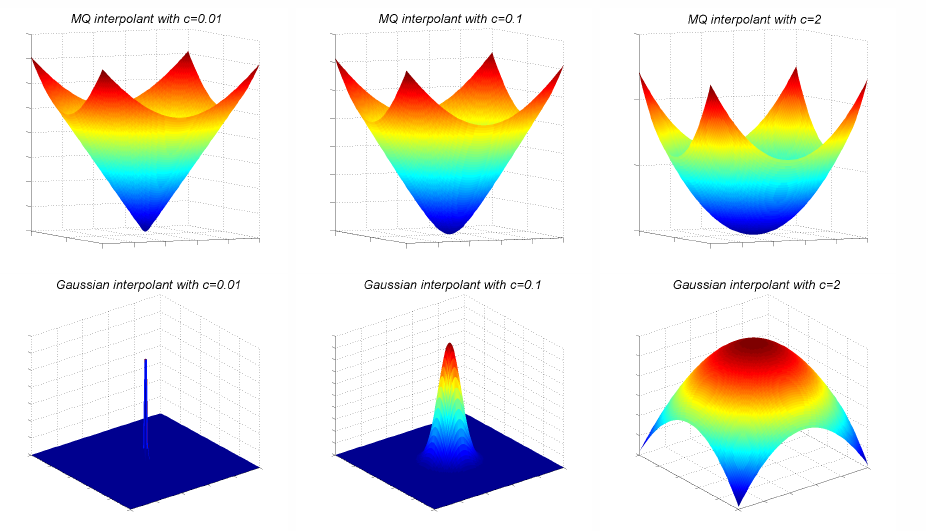
\includegraphics[scale=0.5]{RBFShapeParameters.png}
\captionsource{The Effect of Shape Parameter c on the Gaussian and Multiquadric Radial Basis Functions}{ Y. Zhao (2017) \cite{mski0} page 21}
\label {fig:shape}
\end{figure}

It has been shown in T. A. Driscoll and B. Fornberg.(2002) \cite{rbf4} (amongst others), that a larger value of c will increase accuracy but exceed a limit and the system will become ill conditioned and unstable. Likewise reduceing c will improve the conditioning but also lead to an inaccurate solution. There has been significant effort devoted to finding the optimal value of c for different RBFs however this is still considered an solved problem within the field \cite{mski0}.

\subsection {Ansiotropic Radial Basis Functions}

If the domain of interest is not the same size in all dimensions then an RBF becomes ansiotropic. To model this let $\phi(||\dot -x_{i})$ be some RBF centred around $x_{i} \in \mathbb{R}^{d}$ and $A \in \mathbb{R}^{d x d}$ is an invertible transformation matrix, then the ansiotropic radial basis function $\phi_{A}$ is defined by:
\begin{equation}
\phi_{A}(||\cdot-x_{i}||)=\phi(||A(\cdot-x_{i}||)
\end{equation}
Furthermore we can then define the Ansiotropic Tensor Based Product Function (ATBPF) of the MQ and Gasussian basis functions respectively, as:

\begin{equation}
\phi_{A,x_{i}}(x)= \prod^{d}_{k=1}\sqrt{A^{2}_{k}(x_{k}-x^{k}_{i})^{2}+c^{2}_k}
\end{equation}

\begin{equation}
\phi_{A,x_{i}}(x)= \prod^{d}_{k=1}\exp{\frac{-A^{2}_{k}(x_{k}-x^{k}_{i})^{2}}{ c^{2}_k}}
\end{equation}
Where, k is the $k^{th}$ dimension of x and $A_{k}$ is $k^{th}$ diagonal element of $A \in \mathbb{R}^{d} x \mathbb{R}^{d}$.\\

Whilst we can observe that the Gaussian ATBPF still belongs to the family of RBFs, the MQ ATPBF is no longer radially symmetric.\\

Now, if we let $Ch_{k} = c_{k} / A_{k}$ we find...

\begin{equation}
\phi_{A,x_{i}}(x)= \prod^{d}_{k=1}\sqrt{(x_{k}-x^{k}_{i})^{2}+Ch^{2}_k}
\end{equation}

\begin{equation}
\phi_{A,x_{i}}(x)= \prod^{d}_{k=1}\exp{\frac{(x_{k}-x^{k}_{i})^{2}}{ Ch^{2}_k}}
\end{equation}

... that $Ch_{k}$ represents a 'shape parameter' as noted previously where $h_{k}$ represents the distance between nodes in the kth direction and $A_{k}$ is the number of nodes in that same direction minus one.\\

The first and 2nd derivatives of the ATPBFs are then in the Mutliquadric case,

\begin{equation}
D_{x_{p}}(\phi_{A,x_{i}})=\frac{x_{p}-x^{p}_{i}}{\sqrt{(x_{p}-x^{p}_{i})^{2} + (Ch_{p})^2 }} \prod^{d}_{k\neq p}\sqrt{(x_{k}-x^{k}_{i})^{2}+Ch^{2}_k}
\end{equation}
\begin{equation}
D_{x_{p}}^{2}\phi_{A,x_{i}}(x)=\frac{(Ch_{p})^{2}}{[(x_{p}-x^{p}_{i})^{2} + (Ch_{p})^2 ]^{3/2}} \prod^{d}_{k\neq p}\sqrt{(x_{k}-x^{k}_{i})^{2}+Ch^{2}_k}
\end{equation}
and in the Gaussian case
\begin{equation}
D_{x_{p}}(\phi_{A,x_{i}})= -\frac{2(x_{p}-x^{p}_{i})}{(Ch_{p})^{2}} \prod^{d}_{k=1}\exp{\frac{(x_{k}-x^{k}_{i})^{2}}{ Ch^{2}_k}}
\end{equation}
\begin{equation}
D_{x_{p}}^{2}\phi_{A,x_{i}}(x)= -(\frac{2}{(Ch_{p})^{2}} + \frac{4(x_{p}-x^{p}_{i})^{2}}{(Ch_{p})^{4}}) \prod^{d}_{k=1}\exp{\frac{(x_{k}-x^{k}_{i})^{2}}{ Ch^{2}_k}}
\end{equation}


It can be shown (Y. Zhao (2017) \cite{mski0} p25-26),  that for higher dimensional problems we can use the tensor product of ATBPFs to find:

\begin{equation}
(\Phi)^{-1}=(\Phi_{1})^{-1} \otimes ... \otimes  (\Phi_{d})^{-1}
\end{equation}

\begin{equation}
\lambda = (\Phi)^{-1} \cdot y
\end{equation}

Here, Zhao makes some important points:
Inverting $\Phi$ matrix would cost $O(N^{6d})$
For $\Phi{i}$ this becomes $O(N^{6})$
and the Kroencker Product is $O(N^{2d})$

Therefore potentially using ATPBFs produces some good performance benefits over and above summing RBFs when scaling in multiple dimensions.\\

Whilst Zhao also discussed convergence he also notes there is no current theoretical proof of the convergence of MuSiK-c however his numerical experiments do demonstrate that it does.

\subsection{Kansa method} \label{Kansa}

Kansa's method (E. J. Kansa. (1990)\cite{rbf1}\cite{rbf2}) is a spectral method of approximating u(x) via:

\begin{equation} \label{eq:RBFA}
\hat u(x) = \sum^{N}_{i=1} \lambda_{i} \Phi(||x - x_{i})
\end{equation}

Where $\Phi$ is the radial basis function of choice.

For Kansa's method we choose a $\Xi = \Xi_{1} \cup \Xi_{2}$ which we will call central nodes and where $\Xi_{1} \in \Omega$ (i.e are interior points) whilst  $\Xi_{2} \in \partial \Omega$ exist on the boundary denoted by $\partial \Omega$.

The key of course, is to find the $\lambda$ coefficients for each of the summation terms that make the best approximation of the function u(x). For the elliptical PDE of (\ref{EPDE}) we can substitute (\ref{eq:RBFA}) into the boundary counditions (\ref{eq:EPDE1}) and (\ref{eq:EPDE2}) to get:

\begin{equation} \label{eq:Kansa1}
\sum_{i=1}^{N} \lambda_{i} L \phi_{x_{i}}(x_{j}) = f(x_{j}),\mbox{for j = 1,2,...n}
\end{equation}

\begin{equation} \label{eq:Kansa2}
\sum_{i=1}^{N} \lambda_{i} \phi_{x_{i}}(x_{j}) = g(x_{j}),\mbox{for j = n+1,n+2,...N}
\end{equation}

Which as a matrix system can be represented as:


\begin{align*}
\begin{bmatrix}
 L \phi_{A,x_{1}}(x_{1}) &L \phi_{A, x_{2}}(x_{1}) &... &L \phi_{A, x_{N}}(x_{1})\\
 L \phi_{A, x_{1}})(x_{2}) &L \phi_{A, x_{2}}(x_{2}) &... &L \phi_{A, x_{N}}(x_{2})\\
\vdots &\vdots &\vdots &\vdots\\
 L \phi_{A, x_{1}})(x_{n}) &L \phi_{A, x_{2}}(x_{n}) &... &L \phi_{A, x_{N}}(x_{n})\\
 \phi_{A, x_{1}})(x_{n+1}) &\phi_{A, x_{2}}(x_{n+1}) &...  &\phi_{A, x_{N}}(x_{n+1})\\
\vdots &\vdots &\vdots &\vdots\\
 \phi_{A, x_{1}})(x_{N})  &\phi_{A, x_{2}}(x_{N}) &...  &\phi_{A, x_{N}}(x_{N})
\end{bmatrix}
\begin{bmatrix}
\lambda_{1}\\
\lambda_{2}\\
\vdots\\
\lambda_{n}\\
\lambda_{n+1}\\
\vdots\\
\lambda_{N}
\end{bmatrix}
=
\begin{bmatrix}
f_{1}\\
f_{2}\\
\vdots\\
f_{n}\\
g_{n+1}\\
\vdots\\
g_{N}
\end{bmatrix}
\end{align*}\\


Whilst much work using collocation with RBFs had been performed using Kansa's method to solve elliptic boundary value problems, it wasn't until Myers et al. \cite{rbf0} proposed the space time method that applications for parabolic problems were first successfully investigated.


\subsection{Myer's Space-time method}

In a parabolic problem with a spacial domain $\Omega \in \mathbb{R}^{d}$ and a time domain $t \in [a,b]$ if we let $\Omega_{t} = \Omega x t \in \mathbb{R}^{d} \times [a,b]$ then $\partial \Omega_{t}$ represents the portion of $\Omega_{t}$ that is the boundary.
If the centre nodes $\Theta \in \Omega_{t}$ and $\Theta = \Theta1 \cup \Theta2$ then $\Theta1$ are the nodes in $\Omega_{t}$ excluding $\partial \Omega_{t}$ and $\Theta2$ are the nodes on the boundary $\partial \Omega_{t}$. As with the elliptical PDE, we can show our boundary value problem as:
\begin{equation}
L_{t} = f, \mbox{ within } \Omega \mbox{ excluding } \partial \Omega_{t}
\end{equation}
\begin{equation}
u = g, \mbox{ on } \partial \Omega
\end{equation}
In this case $L_{t}$ is the parabolic operator whilst f and g are the boundary functions that ensure u satisfies the PDE.\\

As with the elliptical problem in \ref{eq:Kansa1} and \ref{eq:Kansa2}, we can now use Kansa's method to solve this system


\subsection{Spectral Methods and the Gibbs phenomena}

The Gibbs phenomenon is a peculiarity of piecewise functions:- any function that is a combination of one or more sub-functions such as a Fourier Series or in our case RBF or ATBPFs. In particular the nth combination of a piecewise function that is continuously differentiable will show persistent oscillatory characteristics in the near region of a discontinuity.These oscillatory overshoots do not reduce as n increases but do approach a finite limit. For example with the classic Fourier Series see \ref{fig:FS} large oscillations are inherent when approximating a digital signal.\\

\begin{figure}[h]
\centering
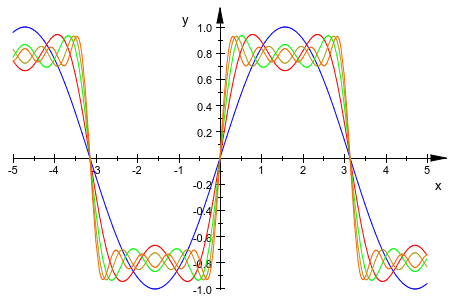
\includegraphics[scale=0.5]{GibbsPhenomenon.png}
%\caption {The Gibbs Phenomenon Obversed During Fourier Series Approximation of a Digital Signal}
%\source{ https://uk.mathworks.com/help/symbolic/mupad\_ug/advanced-plotting-principles-and-first-examples.html }
\captionsource{The Gibbs Phenomenon Obversed During Fourier Series Approximation of a Digital Signal}{ https://uk.mathworks.com/help/symbolic/mupad\_ug/advanced-plotting-principles-and-first-examples.html}
\label {fig:FS}
\end{figure}

In our application, the price of a European Call Option tends toward a discontinuity around the strike price as time approaches expiry as per figure \ref{fig:EuroCall} so naturally there we need a method to over come it which we will take a brief look at in the next section.\\

\begin{figure}[h]
\centering
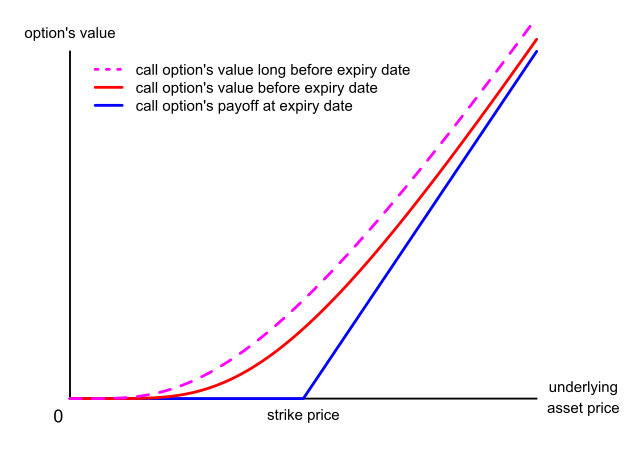
\includegraphics[scale=0.4]{EuroCallOptionPrice.png}
%\caption {The Evolution of European Call Option's Price as Time approaches Expiry}
%\source{ https://commons.wikimedia.org }
\captionsource{The Evolution of European Call Option's Price as Time approaches Expiry}{ https://commons.wikimedia.org}
\label {fig:EuroCall}
\end{figure}


\subsection{Method of Lines}
Here will briefly discuss the Method of Lines (MoL) and how it is used here, but for a complete reference see G. Meyer (2014) \ref{meyer2014time} or Y. Zhao (2017) \cite{mski0}. MoL is a PDE solving technique, where all but one dimension is discretised with the last left to be continuous. In Zhao's approach, the PDE is converted into a set of ODEs which are then solved via RBF interpolation and then a Crank-Nicholson Scheme \cite{mski0} pages 33-34. By careful measurement of the system's Gamma and Speed the time-stepping algorithm is employed to find a point in time (known as T-done) whereby the fitted curve is sufficiently smooth so as to avoid Gibb's effects. The resulting data points are then known as 'smooth initial' data throughout the rest of this paper. As a consequence, the main algorithms presented here (SiK-c and MuSik-c) are in-fact implemented in conjunction with this and other methods as shall be seen.

\subsection{Sparse Grid Collocation}

As described earlier in \ref{Kansa}, it is relatively easy to use RBF interpolation in higher dimensions, but as mentioned in T. A. Driscoll and B. Fornberg.(2002) \ref{rbf4} the distance between nodes must be fixed in order to maintain accuracy. Therefore as the number of dimensions increases, the number of nodes (and hence the number of computations) increases proprotionally to $N^{d}$ where N is the number of equi-distant points in the mesh. This phenomena is sometimes referred to as the curse of dimensionality, the concept that either the amount of computation or the space requirements of an algorithm increase exponentially with the number of dimensions.\\

Whilst the original ideas around Sparse grid Interpolation Kernels (SiK) originated in the Soviet Union\cite{sik1}\cite{sik2} during the 1960s, it wasn't until Zenger's (1991) \cite{sik3} work that the use of sparse grids in PDE solvers really gained traction. Zenger's method relies on the ideas set out in \ref{} ATRBF to save large amounts of space and computation.\\

A detailed explanation of sparse grids is beyond the scope of this paper, Zhao \cite{mski0} (Chapter 4) gives a good description applied to SiK-c and MuSiK-c whilst Subhan \cite{mski} gives a more complete treatment.\\

To begin with, lets define the vector $l = (l_{1}, l_{2}, ... l_{d})$, where $l_{n} = n + (d - 1)$, n is the serial level and d is the number of dimensions. Then a sub-grid $G_{l}^(n,d)$ will contain $N^l{l} = {2^{l_{1}} + 1, ... 2^{l_{d}}}$ points in each direction. When each point point is combined into d-dimensional space the resulting number of nodes N, is:

\begin{equation}
N_{l}^{n,d} = \prod N^{l} = \prod^{d}_{i=1}(2^{l_{i}} + 1)
\label{NMatrix}
\end{equation}
One sparse grid $G^{n,d}$ at level n, dimension d can be expressed as the union of all possible sub-grids $G_{l}^{n,d}$
\begin{equation}
G^{n,d} = \bigcup_{l_{1}=n+(d-1)} G_{l}^{n,d}
\label{SparseGrid}
\end{equation}

Zhao gives the example on page 44 \cite{mski0} of the decomposition of sparse grid $G^{4,2}$, level 4 with 2 dimensions:

\begin{equation}
G^{4,2} = \bigcup_{l_{1}+l_{2} = 5} G^{4,2}_{l_{1},l_{2}}
\end{equation}

Which visualised in 2 dimensions looks like figure \ref{fig:union}
\begin{figure}[h]
\centering
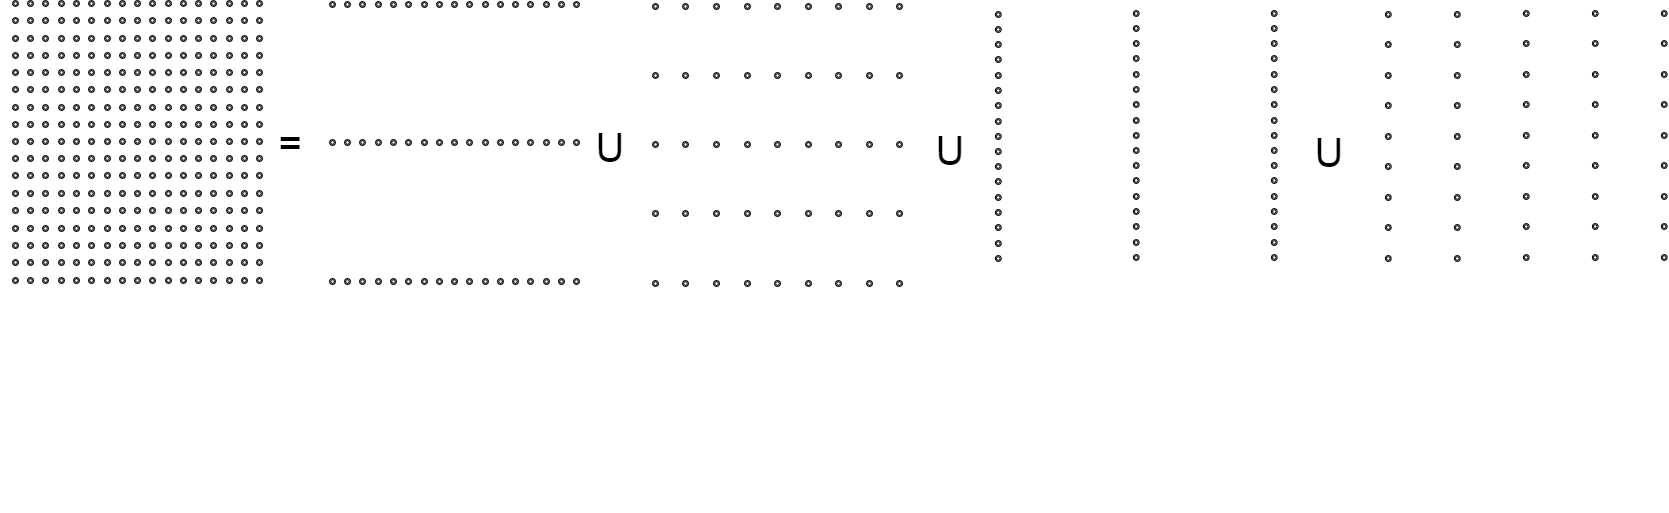
\includegraphics[scale=0.2]{UnionAll.png}
\caption {Sparse grid $G^{4,2}$ is the Union of 4 sub-grids}
\label {fig:union}
\end{figure}

Zhao then speaks about removing duplicates \cite{misk0} pages 48-49, but a union in the strictest sense ignores duplicates in the first place. Ultimately however, he identifies that the total number of nodes per full grid in SiK-c is $O(2^{dn})$ over $O(N^{d})$ for a full grid. Then combined with the multi-level nature of and the space-time method in MuSiKc we end up with $O(Nlog^{d}(N))$\\

Finally, of note is the combination technique to construct the final approximation as equation\ref{comb}.
\begin{equation}
\hat u^{n,d}(x) = \sum^{d-1}_{q=0}(-1)^q \binom{d-1}{q} \sum_{l_{1}=n+(d-1)-q} \hat u_{l}^{n-q,d}(x)
\label{comb}
\end{equation}
\newpage

\section{Implementation Details}
The implementation of the algorithms described above (and detail in appendices \ref{appSiK} and \ref{appMuSiK} ), were originally written in MatLab with parrallel extensions for CPU processing and unfortunately only computes solutions to 1-dimensional (i.e. single asset) European Call Options. In order to expand this codebase (further more referred to as cMuSiK.m and cSik.m) to handle multiple dimensions and scale the available processing power across CPUs and GPUs a two step strategy was undertaken.\\

\renewcommand{\labelenumi}{\arabic{enumi}}
\begin{enumerate}
\item Convert the MatLab code into C++ in one go
\item Evolve parts of the C++ code into C++ CUDA as an ongoing process
\end{enumerate}

As C++ is a versatile multi-paradigm language with good performance capabilities, we can be relatively confident of improving both the maintainability of the codebase whilst keeping the performance without too much micro-optimisation. Additionally C++ is sufficiently close to the native language of NVidia's CUDA that the transition from step-1 to step-2 should be relatively easy. Also the available skills base for C++ is quite high, meaning that the resulting codebase should be easier for others to understand and improve.\\

For the purposes of step-1 C++11 was used primarily for it's in built support for threading and the environment of Microsoft's Visual Studio 2017 due to the familiarity of the author and it's availability as a free tool-set. Care was taken to ensure no platform specific libraries were used such that compilers other than Microsoft's implementation should easily be able to compile the codebase given an appropriate build system. The resulting Visual Studio Solutions, a mixed C++ and CUDA implementation (refered to as SparseGridCollocation.sln) and a pure C++ implementation (referred to as SparseGridCollocationCPP.sln) are the results of this conversion process.\\

In both solutions the code is generally arranged within a namespace heirachy and seperated into sub-projects:\\
%\begin{itemize}
		Organisation:\quad \quad \quad \quad \quad \quad Leicester\\
		Research area:\quad \quad \quad \quad \quad \quad \quad \quad SparseGridCollocation\\
		Program sub system:\quad \quad \quad\quad \quad \quad \quad \quad\quad \quad ProjectSpecific\\
%\end{itemize}
\\Specific functions and classes within the solution will be referred to by the Namespace::Class::Function convention i.e,\\
\begin{itemize}
\item Leicester::SparseGridCollocation::Algorithmn::MuSiKc() refers to the main entry point of the MuSiKc implementation, whilst 
\item Leicester::Common::printMatrix() refers to a particular helper function that prints the contents of a matrix to a string.
\end{itemize}

Each subproject will compile into a separate dynamically linked library (.dll) or an executable program (.exe). For C++ specific code (i.e. projects containing files with extensions .cpp and .h) the msvc compiler will perform the compilation and linking whilst CUDA specific projects (extensions .h or .cuh and .cu) are handled by the NVidia nvcc compiler. Details of both these compilers and their respective software development kits (SDKs) can be found within the appendix.\\

\subsection{Reverse Engineering via Unit Testing}
A common method known within the software engineering community to reverse engineer computer programs who's source code is unavailable is the process of black-box unit testing\cite{comp1}. This is the process of treating the program as a 'black-box' where the true functionality of a particular program can be revealed by carefully selecting the input to the program and measuring the resulting out puts.\\ 

For example if we input the full range of integers into a black-box and observe the results to be squares of the input then we can be reasonably confident that the program implements $F(x) = x -> x^{2}$\\

Whilst in our case the source code is available, this technique can still provide us with a method of measuring and detecting any difference in functionality between our new C++ code and that of the original MatLab code.



\subsection{Eigen API and MatLab comparison}
Eigen\ref{Eigen} is a useful library that styles itself as a 'C++ template library for linear algebra: matrices, vectors, numerical solvers, and related algorithms.' which is open source and distributed under an MPL license. What makes this particular library stand out from others is its coverage of MatLab functions. In particular Zhao makes use of the following MatLab functionality that Eigen also replicates:

\begin{itemize}
\item Linspace - create a linearly spaced vector within a range for a certain number of points
\item zeros, ones and fill
\item size
\item Column \& Row addressing
\item row wise and column wise sum
\item Meshgrid
\item LU decomposition
\item LU Solver
\end{itemize}

A full list of MatLab emulated functionality can be found within the documentation\ref{Eigen1}\ref{Eigen2}.

\subsection{Column Major Format}\label{CMF}
There are two main methods for representing a Matrix within computer memory row-major and column-major formats. With both, each element within the matrix is mapped to an element within contiguous memory. The difference between them however is the exact mapping between those rows and columns and the consecutive elements within memory. It is therefore worth descibing in some detail the exact differences and the convention used here.

An array of values (for example the values 1,2,3...n) are normally stored as consecutively at equally spaced addresses within computer memory, this is known as contiguous memory. If the first element is stored at address A and the size of each value is x, then for element n within an array of length N, the nth element is stored at A + (x * n).

\begin{figure}[h]
\centering
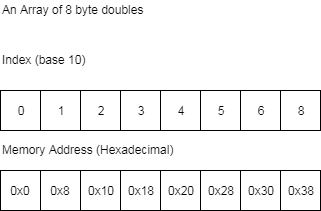
\includegraphics[scale=0.5]{ContiguousArray1.png}
\caption {Contiguous Array}
\label {fig:cont}
\end{figure}

In row-major format each row is appended to the array, with each row element at consecutive locations

\begin{figure}[h]
\centering
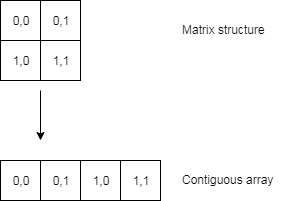
\includegraphics[scale=0.5]{RowMajorFormat1.png}
\caption {Row-Major Format}
\label {fig:rowmajor}
\end{figure}


In column- major format each column element is at a consecutive location, while each column is proceedingly appended to the end of the array

\begin{figure}[h]
\centering
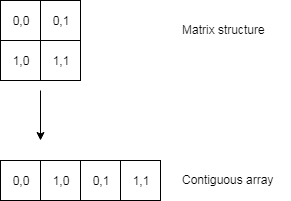
\includegraphics[scale=0.5]{ColumnMajorFormat1.png}
\caption {Column-Major Format}
\label {fig:colmajor}
\end{figure}

The convention used within this project is column-major format, which is the same method as both the Eigen library and that of MatLab. Unfortunately the array construct in C and C++ is simply a pointer to the first element and no further information is provided. Consequently unless the dimensions of an array are known at compile time, for example:

\begin{lstlisting}[language=C++]
int m[] = int[10];
\end{lstlisting}

or unless the programmer stores the dimensions of a dynamic array:\\

\begin{lstlisting}[language=C++]
int rows =10;\\
int cols = 10;\\
int *m = int[rows*cols];\\
\end{lstlisting}

it is impossible to reconstruct the array or matrix from contiguous memory which has big implications that we will see in section \ref{cuda}


\subsection{Expressions and Lazy Evaluation}

Another advantage of Eigen is a useful optimisation for handling wasteful processing called expression trees, which as a concept are similar to those seen in C\# LINQ or SQL. Designed to reduce the number of repeated parsing of a Matrix or array by the programer, Eigen 'records' at compile time all operations performed on a particular matrix and constructs an 'expression' representing the aggregate.Eigen then generates the optimal code to perform the aggregate operation on the matrix in as few loops as possible. Eigen will often do this as late as possible and when done so at actual run-time is known as Lazy Evaluation.

For example, say the programer wanted to add a constant to each element of a Matrix and then later on in the program square each element and so they might write:


%Matrix m = Ones::(rows, cols);\\
%int c = 1;\\
%\t for (int i =0; i < rows; i++)\\
%	for (int j =0; j < cols; j++)\\
%	{\\
%		m(i,j)	+= c;\\
%	}\\
%.\\
%.\\
%.\\
%for (int i =0; i < rows; i++)\\
%	for (int j =0; j < cols; j++)\\
%	{\\
%		m(i,j)	*= m(i,j);\\
%	}\\
%\\

\begin{figure}[h]
\centering
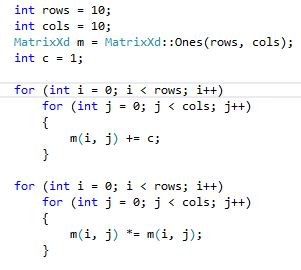
\includegraphics[scale=1.0]{Expressions1.png}
\caption {Inefficient Matrix Parsing}
\label {fig:Expr1}
\end{figure}

In this example it is easy to see that each element of the matrix 'm' is visited by the program twice, but this is obviously wasteful when one considers the following:\\

%Matrix m = Ones::(rows, cols);\\
%int c = 1;\\
%for (int i =0; i < rows; i++)\\
%	for (int j =0; j < cols; j++)\\
%	{\\
%		int a  = m(i,j)	+ c;\\
%		m(i,j) = a * a;\\
%	}\\

\begin{figure}[h]
\centering
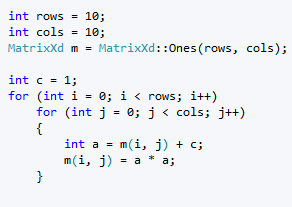
\includegraphics[scale=1.0]{Expressions2.png}
\caption {Efficient Matrix Parsing}
\label {fig:Expr2}
\end{figure}



Where a more efficient programmer will realise that each element of 'm' only needs to be visited once by the program. Eigen's expressions perform the same kind of optimisation when working with Eigen's Matrix template classes, freeing the programmer to concentrate on writing functioning code rather than laboriously optimising their code.

\subsection{Intel Math Kernel Library}
All the algorithms studied within this paper make use of some linear algebra and MuSiK-c in particular uses vector-vector, vector-matrix, matrix-matrix (i.e. BLAS levels 1-3) and LAPACK routines for decomposition and solving linear systems.\\

Whilst it is possible to use Eigen without any further dependency, it is recommend that instead of using it's inbuilt support for BLAS and LAPACK it is best to use a platform specific provider. In our case, we have chosen Intel Math Kernel Library\cite{mkl1} (MKL) which is optimised for Intel based chips\cite{mkl2} and their SSE\cite{mkl4}, SSE2 and SSE3 instructions sets for Single Instruction, Multiple Data\cite{mkl3} (SIMD)\\

Briefly, SIMD allows the processor to stream multiple datasets onto a CPU core in parallel during one instruction. A core is in essence an independent processing unit and modern CPUs are designed to have several of these all on the same chip. What this means is that the same operation can be performed at the same time on several pieces of data simultaneously. Without SIMD that single instruction would need to be executed in serial on each data element individually, which is clearly a vast improvement.\\

This is particularly useful when used in conjunction with multiple threads operating on a multi-core CPU. Each thread of execution operating on a per core basis can process large data sets themselves in parallel giving us effectively two layers of parallelism.

%Both versions of the SparseGridCollocation solution are compiled with the directive EIGEN_USE_MKL_ALL in order to enable useage of MKL, please see the supporting documentation for further reference.


\subsection{Parallelisation with C++ Threading and CUDA}

Whilst one of the main goals of this paper is improve the performance of MuSiK-c via parallelisation, it is important to note that not all algorithmns are can take advantage of such improvements. A program is said to have parallelism or be parallelisable if all or a number of it's operations can occur simultaneously without changing the overall functionality of said program. Otherwise, the algorithm is said to exhibit Sequential behavior.

Taking MuSiK-c as an example (see \ref{appMuSiK}), we see that some sections are inherently sequential (e.g. the need to process each level using the state of prior levels) and some areas can be run in parallel (e.g the interpolation via ATBPFs or RBFs). As multi-threading on the CPU is a well known topic, we will skip this and describe how GPU programing with Nvidia's CUDA achieves massive parallelisation and how CUDALib.vcxproj implements some simple parallel routines.

\subsection {NVidia GPU Hardware architecture}

GPU hardware differs some what from that of CPU architecture figure \ref{fig:CPUGPU} shows how a GPU packs far more cores on to chip than does a CPU. Cores are organised into Streaming Multiprocessors (SM) aka a Warp the GPU equivalent of a CPU's SIMD enabling parallelisation of data flow into and out of the GPU.

\begin{figure}[h]
\centering
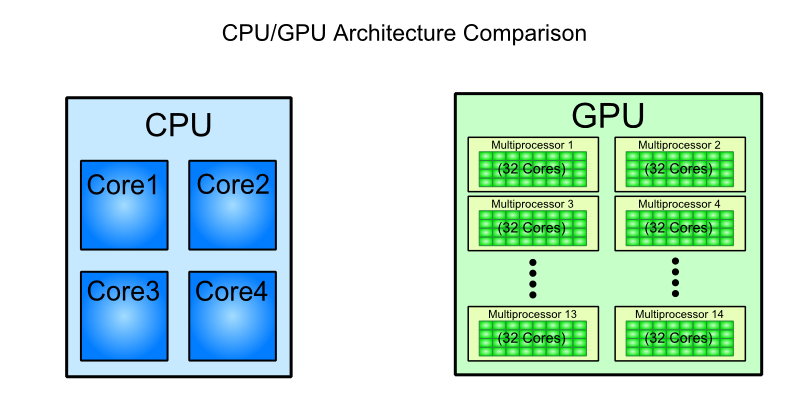
\includegraphics[scale=0.5]{cpu_vs_gpu-1.png}
%\caption {CPU vs GPU Architecture}
%\source{ http://blog.goldenhelix.com/grudy/video-graphics-and-genomics-a-real-game-changer/ }
\captionsource{CPU vs GPU Architecture}{ http://blog.goldenhelix.com/grudy/video-graphics-and-genomics-a-real-game-changer/}
\label {fig:CPUGPU}
\end{figure}

Whilst it might seem from this that GPUs are far superior to CPUs where the are lacking is in the amount of RAM the GPU cores can access. For example the reference hardware in \ref{refH} is a current (as of 2017) GPU containing 2Gb of memory, whereas the CPU (a 2011 vintage) can access the entire 16 Gb of system RAM with ease. As such, to make effective use a GPU's computing power, the CPU must always be busy sending data down the line to the GPU device.

CUDA's threading model is shown in figure \ref{fig:CUDAthread} and like all concurrent execution models, the unit of execution is known as a thread but in CUDA threads are also organised using Blocks and Grids\ref(cuThrd).
\begin{itemize}
  \item Thread: A unit of sequential execution, in CUDA all threads execute the same sequential program in parallel.
  \item Thread Block: A group of threads which all execute on the same streaming multiprocessor. Threads within a block can synchronise with each other and exchange data.
  \item Grid: A group of Thread Blocks where blocks execute across multiple SMs, can't synchronise and communication between is expensive.
\end{itemize}

The CUDA run-time API provides a thread object that allows the programmer to identify the x-y-z 3-dimensional coordinate of the thread within it's block as well as the same data for the block within the grid.

\begin{figure}[h]
\centering
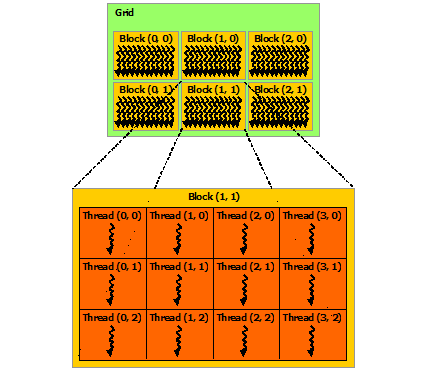
\includegraphics[scale=1.0]{grid-of-thread-blocks.png}
%\caption {CUDA threading model}
%\source{ http://docs.nvidia.com/cuda/cuda-c-programming-guide/index.html }
\captionsource{CUDA threading model}{ http://docs.nvidia.com/cuda/cuda-c-programming-guide/index.htm}
\label {fig:CUDAthread}
\end{figure}


Initally, it seems that CUDA is designed specifically for our purposes: parsing large NxM matrices in parallel. As we can keep track of the Thread's x and y indices within the larger grid and block system we launch a grid with enough blocks and threads (over 10,000 concurrently on the reference hardware alone), to process each element of the matrix in parallel. Likewise as the most efficient method is to use blocks of 32x32 threads we can launch more threads than we need but let some 'out of index' threads process nothing.

In general a CUDA program's functions are organised into 3 main types\ref:{cuPrg} based on whether they are executed on the host-side (the CPU) or the device-side (the GPU):

\begin{itemize}
  \item Kernel: What is termed as the host-side program i.e. operates as a normal C++ program on the CPU able to address system memory and call the Cuda Runtime API
  \item Global Functions: A device-side function that can be called from the Kernel but also from other device-side functions. These functions must be executed by defining grids, blocks and threads that will execute the function concurrently.
  \item Device Functions: Functions that can only be called by device side code and as such themselves run on the device. As with Global Functions must be executed with a declared set of threads.
\end{itemize}

The CUDA runtime is rather limited, in that useful libraries such as the C++ Standard Template Library (STL)\ref{cuSTL} or Eigen are not usable on the GPU. Furthermore the run-time only supports the copying of data from host to device (or device to host) via the use of pointers. Both of these drawbacks present significant problems to the programmer. A matrix therefore must be represented by a pointer construct (hence our explanation or column-major format in section \ref{CMF}) in order to be loaded by the GPU and passed across functions. Likewise once copied back to the host, the pointer array must be mapped back to a matrix structure. For MuSiK-c this means that our dynamically sized matrices are difficult to handle correctly in CUDA unless we pass the dimension sizes around with them. This also complicates (very significantly) the implementation of our grid interpolations as we must keep track of different indices pointing to different elements in our Test Nodes and our Central Nodes.\\

To add further complexity to the mix, imagine you wanted to execute a grid with n blocks of m threads but each thread itself had to spawn another grid of p blocks and q threads. CUDA can do this as well via what it calls \emph{Dynamic Parallelism}\ref{cuDP} an example of which can be seen in CudaLib.vcxproj where $CudaLib::Gaussian2d\_CUDA$ launches $CudaLib::Gaussian2d2\_CUDA$. Dynamic Parallelism is important for applications such as MuSiK-c where there are at least three layers that can be parallelised i.e. ShapeLambda and two levels of RBF Interpolation . The big drawback is that without multiple graphics cards installed on your system, it is not possible to debug these kinds of routines. \\

As a result of the difficulty in indexing dynamically sized matrices in contiguous memory and that the reference hardware only included one CUDA capable GPU, CudaLib works reasonably well for 1 dimensional European Call Options at low levels. However not so for the larger matrices encountered at level 7 and above or for Basket options.


\subsection{CUDA Thrust Library}

CUDA Thrust\ref{cuThrust} is an abstraction over the main CUDA programming model. It in effect allows the user to define their matrices in an STL-like vector container, define a special function called a 'functor' and the thrust library will automatically copy the matrix to the GPU and execute the functor against every element in the matrix. What is especially useful in our case is that the functors are stateful, such that they are defined as a C Struct type allowing us to know within the function body the dimensions of the various matrices that we are processing as well as any further supporting data we may wish to access.


 
\section Computational Experiments
The following experiments are designed to verify the correctness of the new codebase versus that of the legacy MatLab as well as indicate relative performance differences. Each experiment is run twice, once for the pure C++ version and then once for the mixed CUDA C++ version. Full output of each experiment is shown in the appendices.

\subsection{C++ Experiments}
Compiled from Usng SparseGridCollocationCpp.sln, Experiments.vcxproj \\
Run using the command Experiments.exe [experiment number]\\
where [experiment number] corresponds to the sub section number below:

\subsection{Experiment 1}\label{cppExp1}

Purpose: Verification of Method of Lines 1 Dimension in C++ vs MatLab (MOL to find an earlier time) To\_get\_ini.m\\

Viewing the graphical comparison in figure \ref{fig:cppExp1} of MatLab versus our one dimensional Method of Lines implementation shows an exact match, which suggests our implementation is functionally equivalent. We will therefore continue to use this new code to generate the smooth initial data used in the main algorithms.

\begin{figure}[h]
\centering
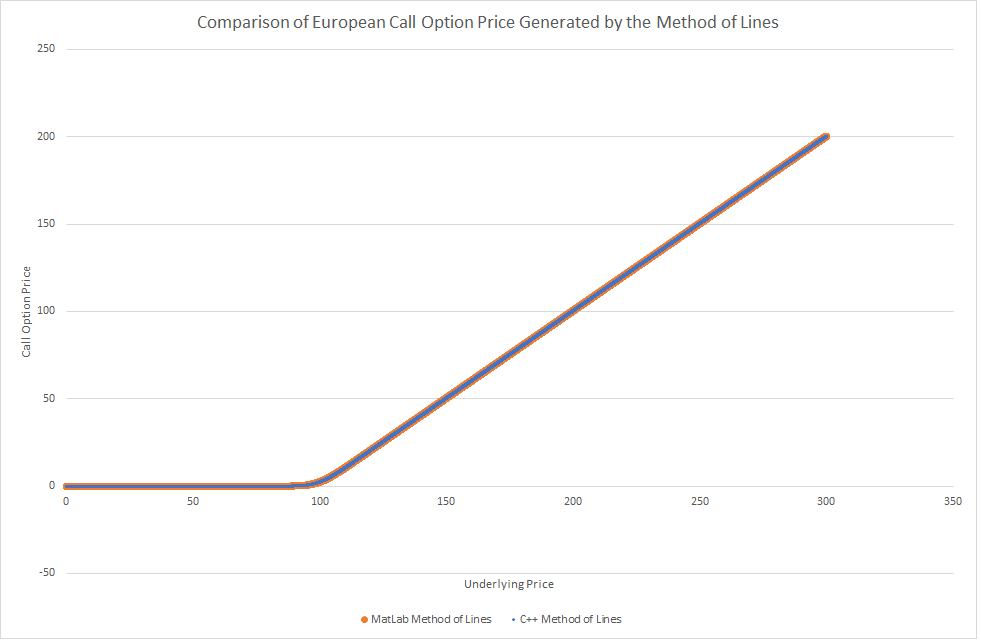
\includegraphics[scale=0.3]{cppExp1-chart.png}
\caption {}
\label {fig:cppExp1}
\end{figure}

\subsection{Experiment 2}\label{cppExp2}

Purpose: Verification of SiK-c 1 Dimension in C++ vs MatLab (sparse grid collocation) cSIK.m\\

In this case the graph \ref{fig:cppExp2} clearly shows a difference in the implementations of SiK-c in C++ and that of the original MatLab code. From \ref{} we would expect to see far smaller Root Mean Squared (RMS) errors than we actually do.

\begin{figure}[h]
\centering
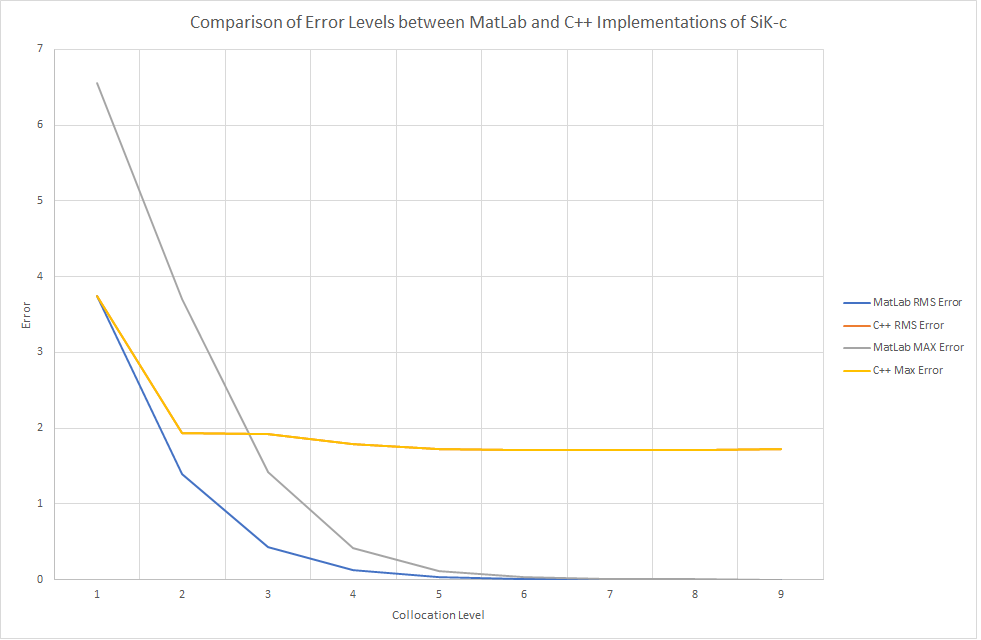
\includegraphics[scale=0.3]{cppExp2-chart.png}
\caption {}
\label {fig:cppExp2}
\end{figure}

\subsection{Experiment 3}\label{cppExp3}

Purpose: Verification of MuSiK-c 1 Dimension C++ vs MatLab (sparse grid collocation) cMuSIK.m\\

Whilst the calculated points may not match, the graph \ref{fig:cppExp3e} shows that even at logarithmic scale the RMS and Maximum errors are almost exact and trending in the same direction, suggesting the C++ version is equivalent

\begin{figure}[h]
\centering
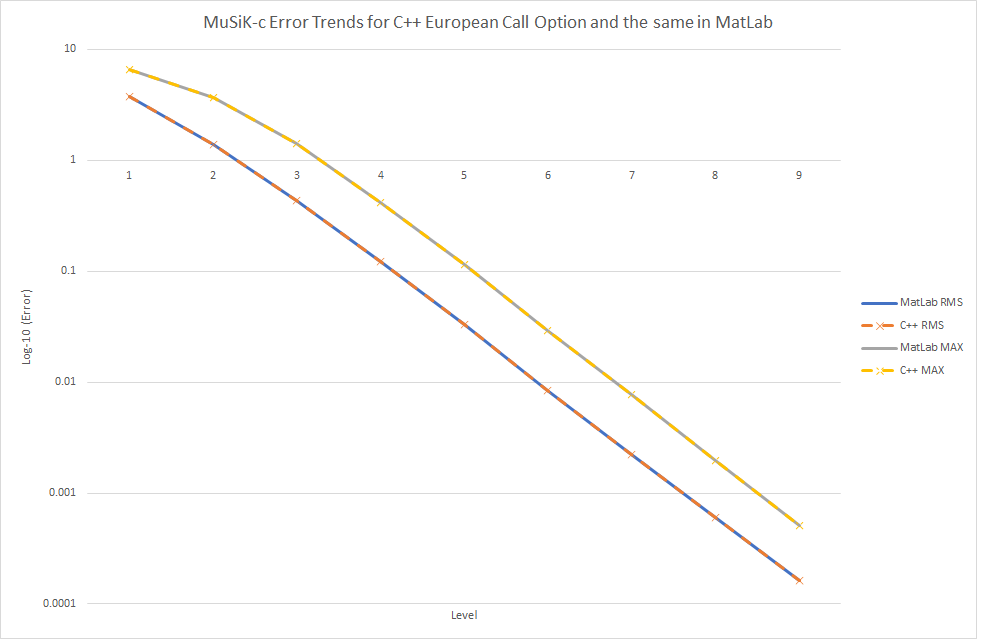
\includegraphics[scale=0.3]{cppExp3-errors.png}
\caption {}
\label {fig:cppExp3e}
\end{figure}

Measuring performance, we can see that C++ outperforms MatLab at lower collocation levels, in this case. This is perhaps partially due to the constant time required for MatLab to launch it's parallel pool. However as no thread pooling is used in the C++ implementation then this is a fair test.

\begin{figure}[h]
\centering
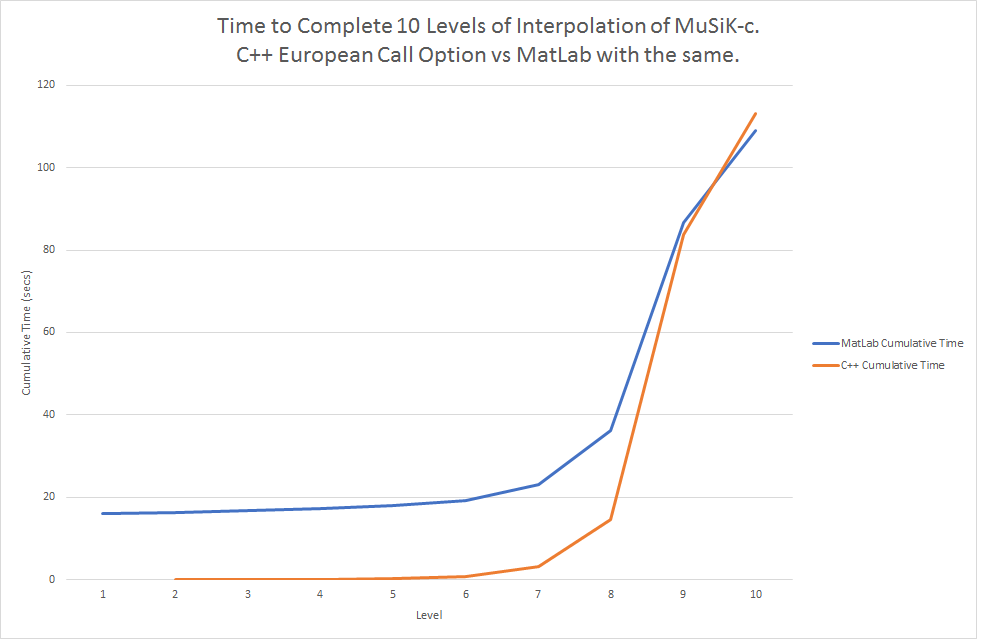
\includegraphics[scale=0.3]{cppExp3-time.png}
\caption {}
\label {fig:cppExp3t}
\end{figure}

\subsection{Experiment 4}\label{cppExp4}

Purpose: Verification of Method of Lines N Dimensions, 1 asset European Basket Call Option in C++ vs MatLab (MoL to find an earlier time) To\_get\_ini.m\\

Now turning to the multi-dimensional versions of our C++ code, we choose a Basket Option with 1-underlying asset, whose pay off is related to the arithmetic mean of the underlying. This means that a 1-asset Basket Call Option should have the same price as a European Call Option on the same asset where the strike prices are the same.

\begin{figure}[h]
\centering
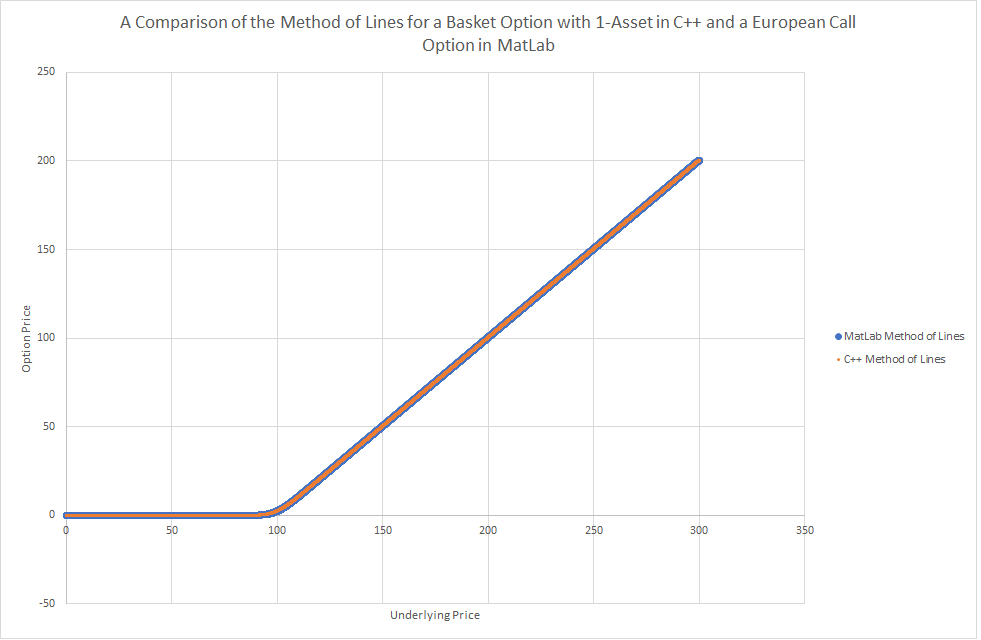
\includegraphics[scale=0.3]{cppExp4-chart.png}
\caption {}
\label {fig:cppExp4}
\end{figure}

Indeed, for our Method Lines in N-Dimensions seems to be equivalent to the same MatLab procedure with same inputs. Usefully we can now use this the output here to feed the other algoirthmns in multiple dimensions.

\subsection{Experiment 5}\label{cppExp5}

Purpose: Verification of MuSiK-c N Dimensions, 1 asset European Basket Call Option in C++ vs MatLab (sparse grid collocation) cMuSIK.m\\

Using the output of the last experiment we now feed the smooth initial data to the main MuSiK-c algorithmn and compare it to MatLab's output. Graph \ref{fig:cppExp5e} shows a continued good match even at logarithmic scale, despite a small (but negligible here) drift upwards in the error as collocation levels increase.

\begin{figure}[h]
\centering
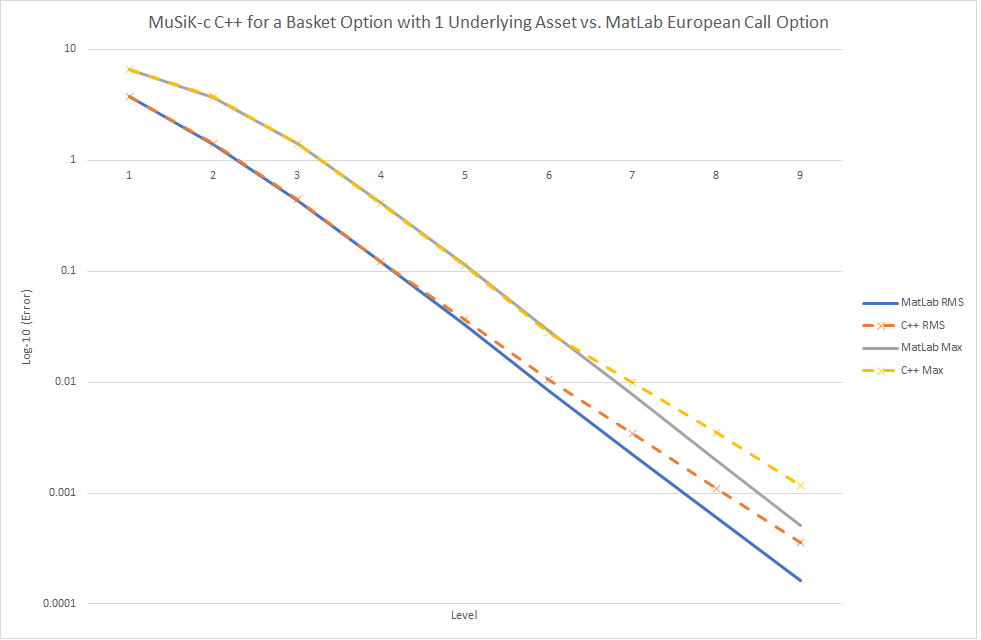
\includegraphics[scale=0.3]{cppExp5-errors.png}
\caption {}
\label {fig:cppExp5e}
\end{figure}

As we saw previously in \ref{Experiment 3} and now in graph \ref{cppExp5t} C++ also outperforms MatLab at lower collocation levels even though it must work a little harder to cater for multiple dimensions.

\begin{figure}[h]
\centering
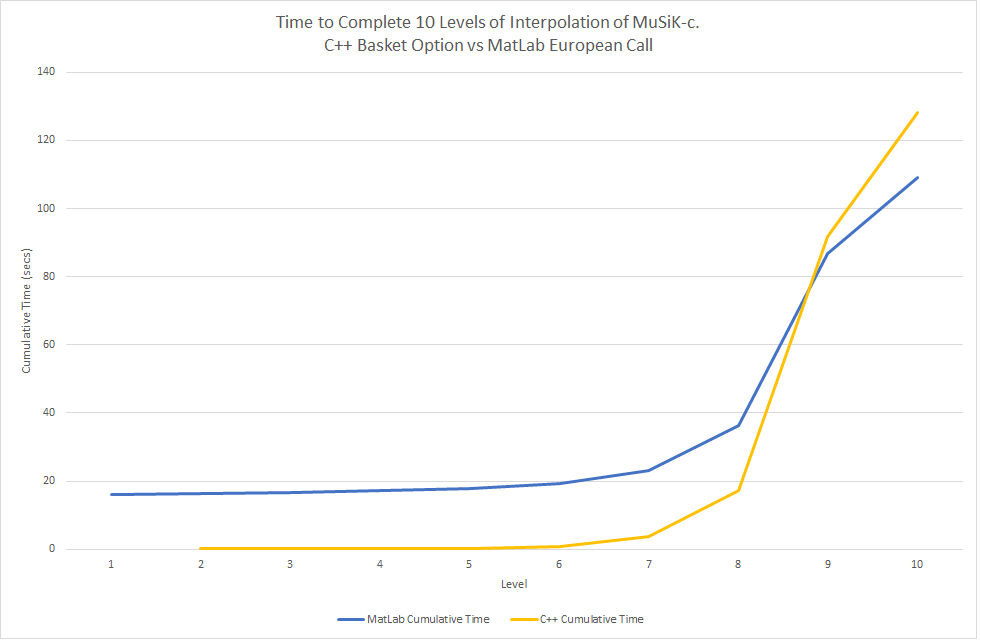
\includegraphics[scale=0.3]{cppExp5-time.png}
\caption {}
\label {fig:cppExp5t}
\end{figure}

\subsection{Experiment 6}\label{cppExp6}

Purpose: Verification of Method of Lines N Dimensions, 2 asset European Basket Call Option in C++ vs QuantLib Montecarlo 2-Asset\\

We are sceptical of how well MoL will scale with extra dimensions and whilst we have already done the work to parallelise RBF/ATBPFs in the main MuSiK-c algorithm the process for finding T-done is inherently sequential and hence slow. Instead, here we will begin testing a more scalable method of generating smooth initial data and make the \emph{big assumption} that T-done for 2 assets is the same as T-done for N-assets: QuantLib's\cite{ql} implentation of a Montecarlo algorithm for basket options.

\begin{figure}[h]
\centering
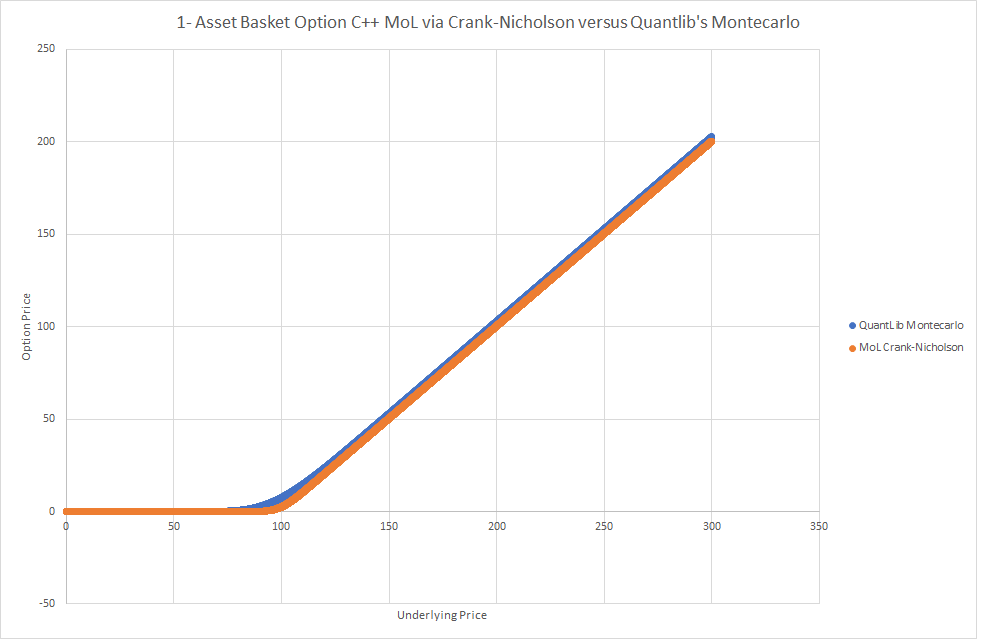
\includegraphics[scale=0.3]{cppExp6-chart.png}
\caption {}
\label {fig:cppExp6}
\end{figure}

Graph \ref{fig:cppExp6}, shows that (as we might have expected) Montecarlo is very close in terms of accuracy to MoL, at least beyond the near region of the strike. Both MuSiK-c and SiK-c rely on the smooth initial data generated here to supplement their calculations close to the boundary represented by T-done, so the selection of T-done using Montecarlo may well have a big effect later on.

\subsection{Experiment 7}\label{cppExp7}

Purpose: Verification of MuSiK-c N Dimensions, 2 asset European Basket Call Option with QuantLib MC as method of choice in C++\\

Extending our Basket Option to 2 Underlying Assets presents a real challenge to our method. Graph \ref{fig:cppExp7e} shows errors only increasing until we reach the cap of the number of levels we chose to run. A cap of 6 levels is made, due to the process using up all available system memory from the 7th level onwards. At this time, we are unsure whether the difference in error is due to our choice of T-done, whether we're not generating the N-matrix (and hence our shape parameters) correctly, there is a bug in the code or there is an inherent problem with MuSiK-c. We could invest in more memory for the reference system or find some memory management improvements to reduce the algorithm's footprint.

\begin{figure}[h]
\centering
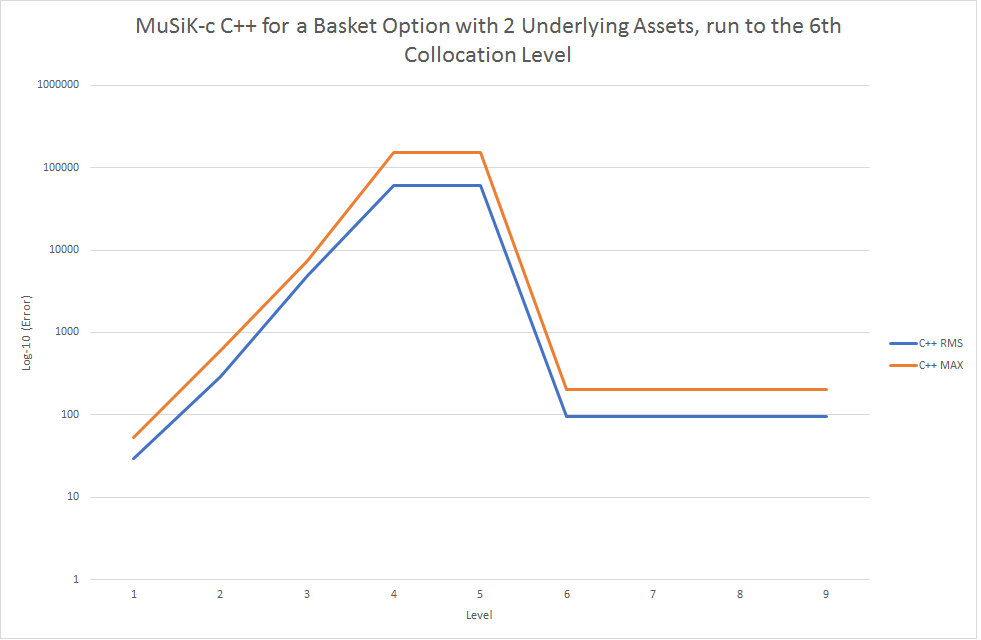
\includegraphics[scale=0.3]{cppExp7-errors.png}
\caption {}
\label {fig:cppExp7e}
\end{figure}

Performance figures in \ref{fig:cppExp7t}, prove to be disappointing.

\begin{figure}[h]
\centering
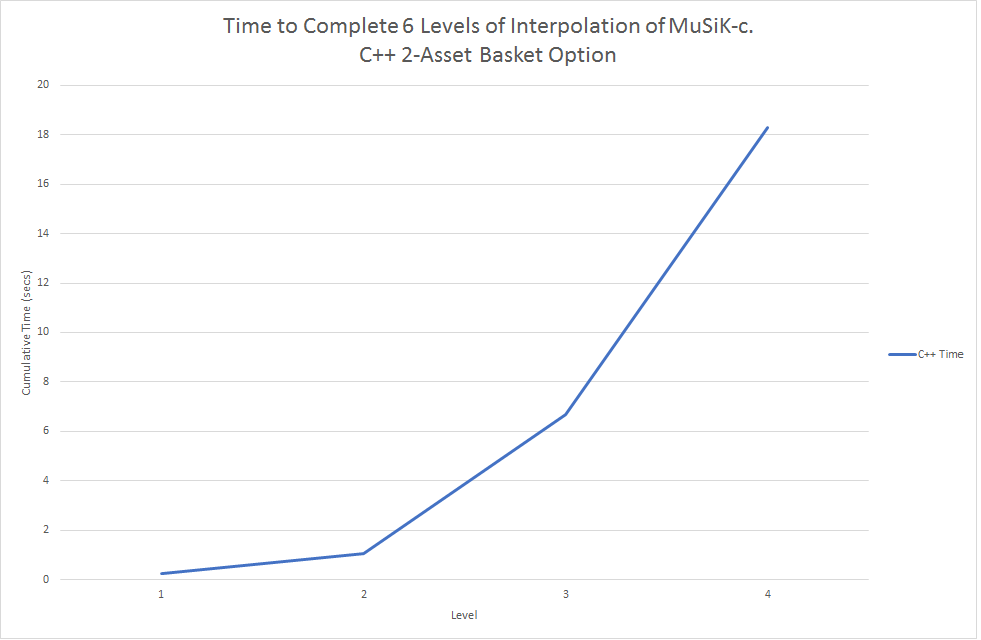
\includegraphics[scale=0.3]{cppExp7-time.png}
\caption {}
\label {fig:cppExp7t}
\end{figure}

\subsection{CUDA \ C++ Experiments}

Compiled from Usng SparseGridCollocation.sln, Experiments.vcxproj \\
Run using the command Experiments.exe [experiment number], 
where [experiment number] corresponds to the sub section number below:


\subsection{Experiment 3}\label{cuExp3}

Purpose: Verification of MuSiK-c 1 Dimension in C++ CUDA vs MatLab (sparse grid collocation) cMuSIK.m\\

We now benchmark our 1-dimensional CUDA C++ implementation with that of the original code. Graph \ref{cuExp3e} shows an exact match between both, so we can verify that this implementation is correct.

\begin{figure}[h]
\centering
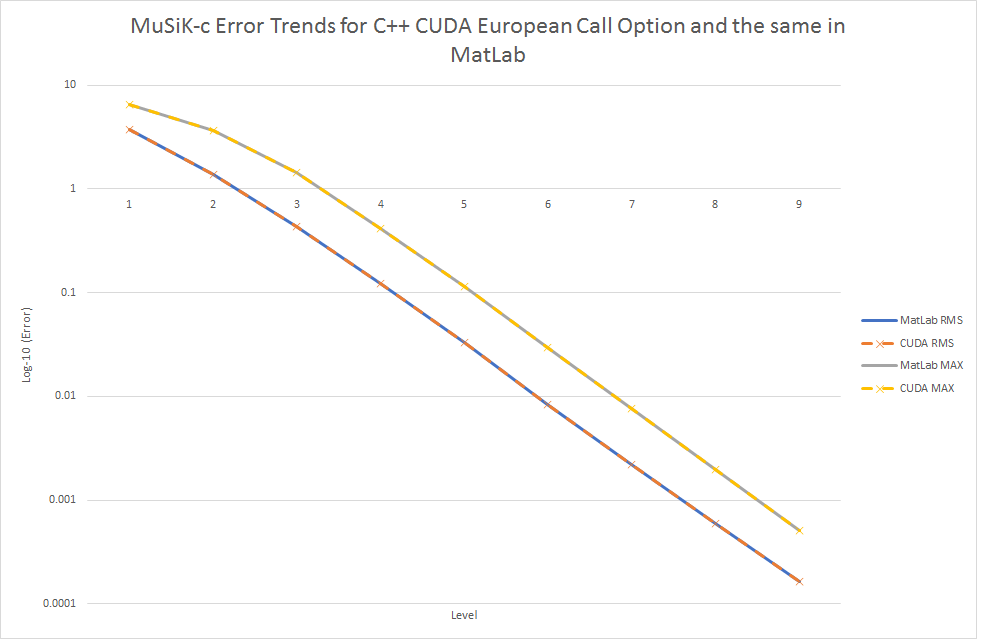
\includegraphics[scale=0.3]{cuExp3-errors.png}
\caption {}
\label {fig:cuExp3e}
\end{figure}

However when we explore performance in the graph \ref{fig:cuExp3t}, we see that the CUDA implementation is significantly slower at higher levels and marginally so at lower ones. Whilst there are 'warm up' costs for launching kernels on the GPU (which perhaps explain the constant difference below level 8), these do not account for the poor performance at higher level.

\begin{figure}[h]
\centering
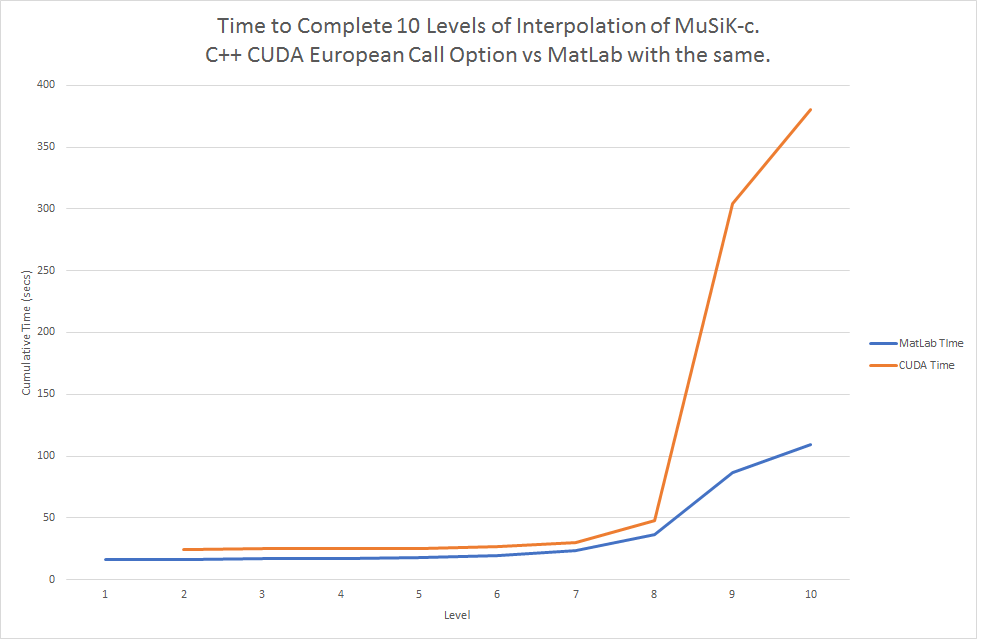
\includegraphics[scale=0.3]{cuExp3-time.png}
\caption {}
\label {fig:cuExp3t}
\end{figure}

\subsection{Experiment 5}\label{cuExp5}

Purpose: Verification of MuSiK-c N Dimensions, 1 asset European Basket Call Option in C++ CUDA vs MatLab (sparse grid collocation) cMuSIK.m\\

As with the equivalent experiment in pure C++ \ref{cppExp3}, graph \ref:{fig:cuExp5e} reveals that our CUDA implementation is in good agreement with the original code. Again we see a slight drift in both RMS and MAX errors once we reach higher levels, which suggests a systematic difference in the way we are calculating the derivatives of the ATBPFs.

\begin{figure}[h]
\centering
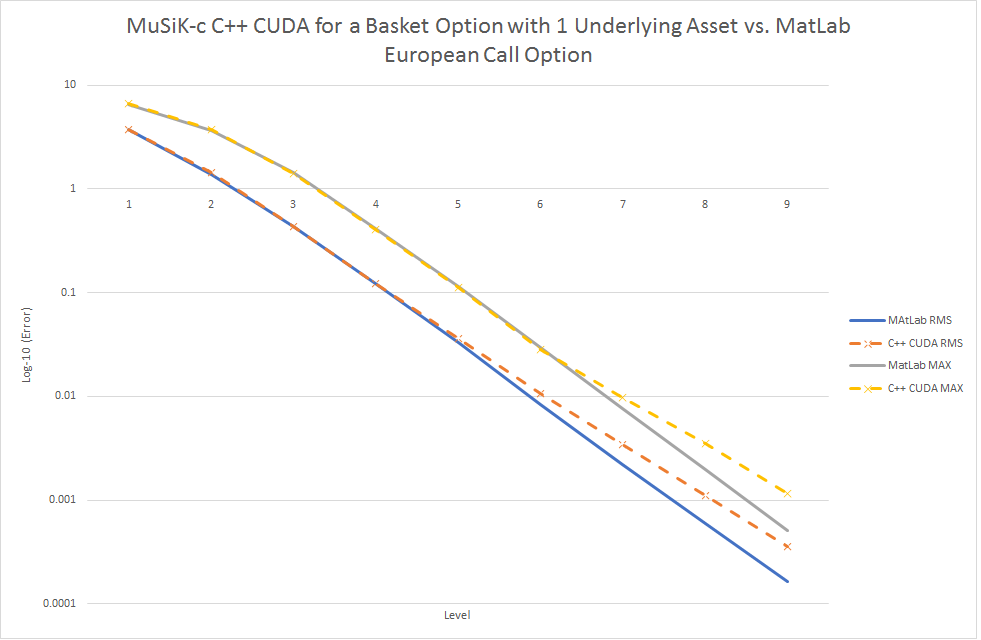
\includegraphics[scale=0.3]{cuExp5-errors.png}
\caption {}
\label {fig:cuExp5e}
\end{figure}

Performance wise, its a similar story to the prior experiment, however CUDA seems to out perform at the lower levels before this advantage receeds at high levels. We know that we've not fully parallelised the PDE-reconstruction (which is used proportionally more at higher levels), in this version of the code so perhaps by doing so we will gain a better advantage.

\begin{figure}[h]
\centering
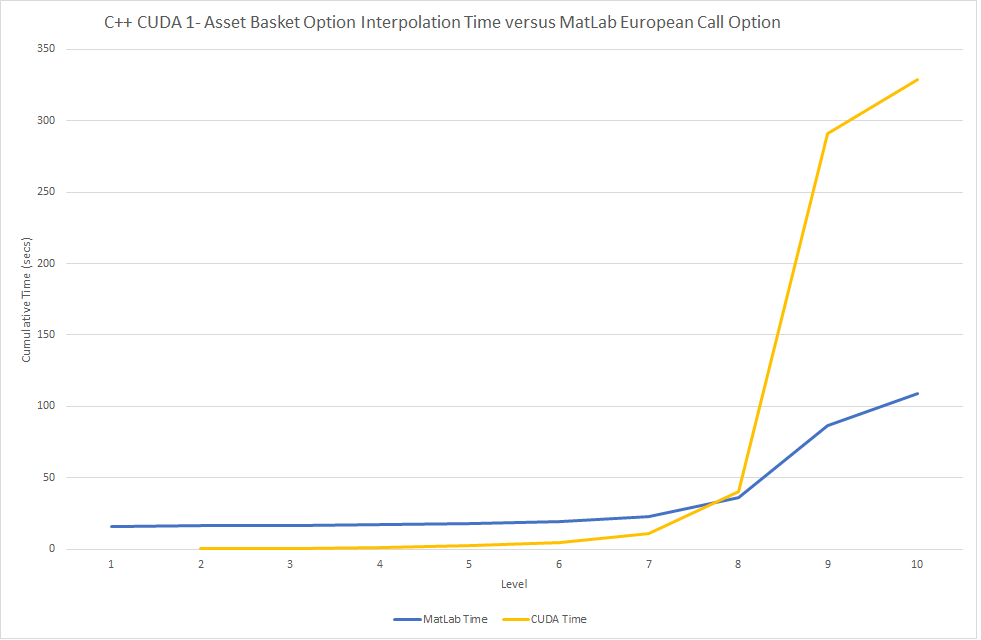
\includegraphics[scale=0.3]{cuExp5-time.png}
\caption {}
\label {fig:cuExp5t}
\end{figure}

\subsection{Experiment 7}\label{cuExp7}

Purpose: Verification of MuSiK-c N Dimensions, 2 asset European Basket Call Option with QuantLib MC as method of choice in CUDA

As with the corresponding pure C++ experiment \ref{cppExp7}, the number of levels are capped to 6 due to the same problems and in addition GPU memory consumption contraints. Graph \ref{fig:cuExp7e}, shows that whilst there is a slight improvement in accuracy at the lowest levels some problem with our program causes the errors to quickly mount up beyond level 2.

\begin{figure}[h]
\centering
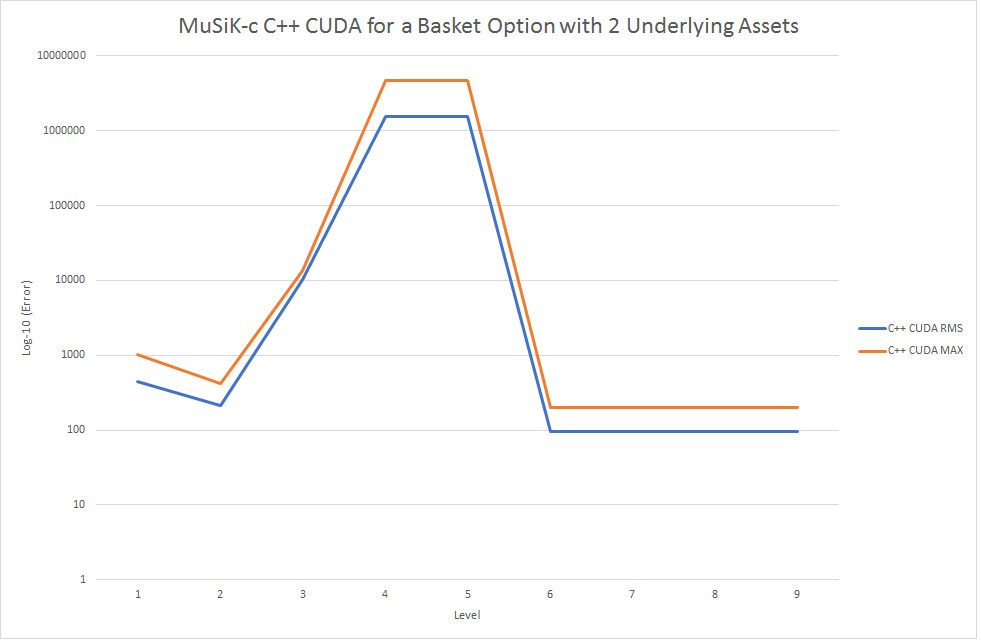
\includegraphics[scale=0.3]{cuExp7-errors.png}
\caption {}
\label {fig:cuExp7e}
\end{figure}

Again, the performance figures shown in \ref{cuExp7t} are disappointing worse so than with 1-asset. However it may be worth investigating if theses only scale linearly with dimensions.

\begin{figure}[h]
\centering
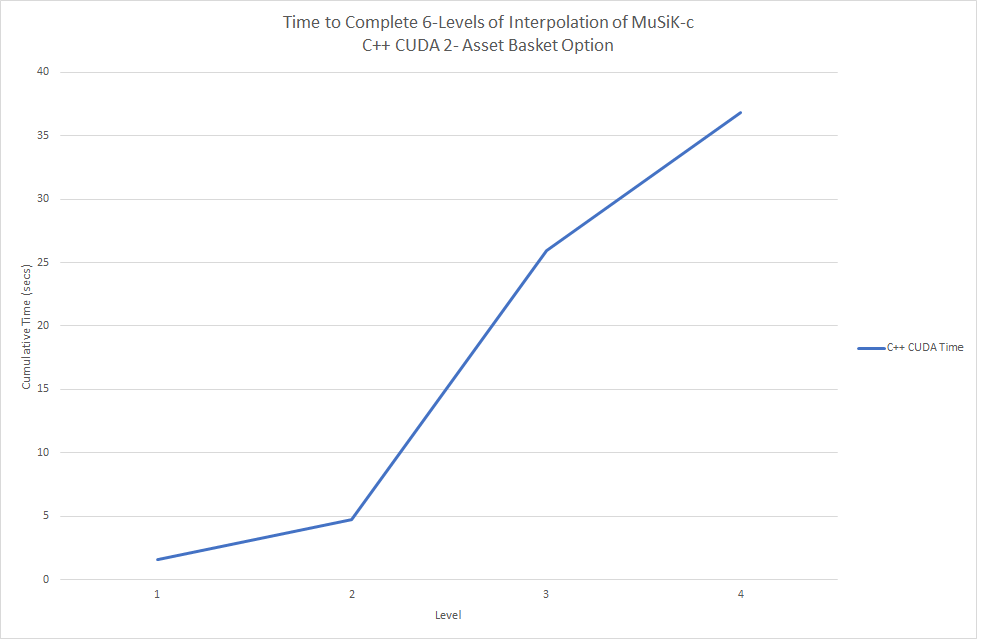
\includegraphics[scale=0.3]{cuExp7-time.png}
\caption {}
\label {fig:cuExp7t}
\end{figure}

\subsection{Profiling Results}
Both versions of the algorithm have been profiled to gain insight into potential bottle necks, for C++ see\ref{prof1} and for the GPU profile of CUDA see\ref{prof2}
Of the 5 hottest functions within our C++ version, 4 are library code (Intel MKL) and the last is our implementation or RBF interpolation. This suggests that we are correct in our assumption that this part of the software is perhaps best run on the GPU.
The CUDA profiler is a little more difficult to read, however the main item is concern is that we seem to be mainly using the default stream processor and the other streams for little else. This potentially is the cause of the helpful warnings at the bottom concerning low through put, memcopy efficiency and low compute.

\newpage
\section {Conclusions}

We have proven that both our C++ and C++ CUDA implementations are functionally equivalent to the original MatLab code in the 1-Asset case for European Call Options developed by Zhao for his PhD. Thesis \cite{mski0}. Further, we have extended his algorithm to cater for Basket Options and other higher-dimensional instruments. Unfortunately we can only prove the correctness of this approach using 1-Asset instruments. 

In terms of hardware and software scalability we have learnt that C++ in conjunction with Eigen and Intel MKL allow us to scale the number of CPUs and size of system Memory reasonably well. However we should note, that a more in depth forensic approach to optimisation should be undertaken before claiming this. In terms of heterogenous programing across both CPU and GPU, we have learnt that significantly more care needs to be taken using and optimising algorithms for NVidia CUDA. Whilst our implemntation does use CUDA, so far we've been unable to push (and remove) enough data from the GPU memory at fast enough rates to really push the reference hardware to it's limits.

\section {Further Work}

As was noted in section \ref{sec:RBF} shape parameters have a significant bearing on the out-come of all RBF interpolants. Whilst it seems that we are using close to the correct method of generating both them and the sub-grids with 1-Asset, this is perhaps not the case with more than 1. There are perhaps 2 approaches to discovering whether this is the case. Firstly we could return to the theoretical background and re-affirm whether we are adhering to the ideas there. Secondly, we could build some automated learning method to scan through a range of shape parameters and discover the optimal values.

We are also unconvinced by our method of choice for generating smooth initial data. As we have seen, the Method of lines does not seem to scale well as dimensions increase. Further more, we have not investigated our alternative Montecarlo approach sufficiently to eliminate any extra problems it might bring to MuSiK-c. In particular, it lacks the ability to find a suitable T-done for RBF interpolation so requires the user to make an 'educated guess' as to where to start MuSiK-c. If this is done incorrectly, the method will encounter Gibb's phenomenon and so lose accuracy close to dis-continuities.

In terms of software, there is plenty of optimisation to be done both in terms of memory footprint (and through put), thread pooling, efficient algorithms and further parallelisation. Each of these areas would need significant attention should this implementation ever be considered for production use. In addition, the unit and regression testing coverage is neither large nor automated in an efficient manner. Addressing that would significantly improve the ability of other code contributors work on the project.

In terms of hardware, we have barely scratched the surface. Whilst this solution has been deployed and run (on occasion with a virtual machine on Google Compute, it has only been run on very limited cloud hardware. GPU enabled servers are available to use for the professional subscriber and in the near future NVidia will launch their on GPU based Grid-Cloud hybrid\ref{cuCloud}. So the project is in a good position to take advantage of new innovations in this space.

\newpage
\section{Appendices}



\subsection{SiK-c Details} \label{appSiK}
The basic Sparse Grid Collocated Interpolation Kernel (SiK-c) is shown in figure \ref{fig:sikc1} is our basic algorithmn which once expanded to multiple levels of collocation becomes MuSiK-c.

\begin{figure}[h]
\centering
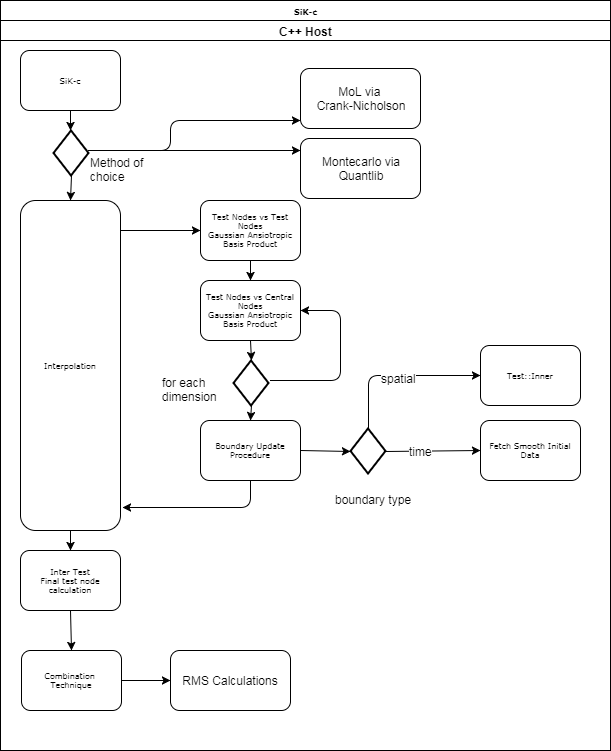
\includegraphics[scale=0.5]{SiKc1.png}
\caption {The SiK-c Algorithmn}
\label {fig:sikc1}
\end{figure}


\newpage
\subsection{MuSik-c Details} \label{appMuSiK}
MuSiKc on the other hand use multi-level co-located interpolation, where the results of each level are re-used as inputs for the next. As such, MuSiK-c is an inherently sequential evolution of SiKc.\\
 The following diagram\ref{fig:musikc1} shows the processing flow of the main algorithm and it's differences to SiK-c.\\

\begin{figure}[h]
\centering
\includegraphics[scale=0.4]{MuSiK-c.png}
\caption {The MuSiK-c Algorithmn}
\label {fig:musikc1}
\end{figure}


\subsection{D. Navigating from Theory to Source Code}
Theoretical points of interest and their C++ implementations

The methods of choice for generating smooth initial data.
\begin{itemize}
\item Method of Lines via Crank-Nicholson Leicester::SparseGridCollocation::MoL::MethodOfLines
\item Montecarlo Leicester::SparseGridCollocation::Montecarlo::BasketOption
\end{itemize}

The generation of N- matrix \ref{NMatrix} and the generation of Test Nodes for each level is implemented within:
\begin{itemize}
\item Leicester::SparseGridCollocation::TestNodes::GenerateTestNodes
\item Leicester::SparseGridCollocation::Interpolation::primeNMatrix
\item Leicester::SparseGridCollocation::Interpolation::subnumber
\end{itemize}

Ansiotropic Tensor Based Product Interpolation Using Gaussian RBFs
\begin{itemize}
\item C++ Leicester::SparseGridCollocation::RBF::Gaussian2D
\item C++ CUDA  Leicester::ThrustLib::GaussianNd1::GaussianNd1
\item General Interpolation and Boundary Update Procedure Leicester::SparseGridCollocation::Interpolation::shapelambdaGeneric
\end{itemize}

\subsection{ Further Information on Automated Testing}

SparseGridCollocation.sln and MuSiKc.m include a number of methods and frameworks in order to isolate particular modules of functionality some of which are:
\begin{itemize}
\item Leicester::SparseGridCollocation::checkMatrix() - Of which there are 3 versions, allowing the user of the function to compare with configurable precision, the sameness of 2 matrices.
\item Leicester::Common::Utility::printMatrix() - Including several variants that will write the contents of a matrix to a string in various formats prior to inserting into cout and printing to the console
\item Leicester::Common::Utility::saveMatrix() - Save the contents of a matrix to a human readable text file
\item Leicester::Common::Utility::saveMatrixB() - Save the contents of a matrix to a binary file so as not to lose precision but the dimensions of the matrix are not saved.
\item WriteAllToFile.m - Save the contents of a matrix to a binary file.
\item TestHarness.vcxproj - Contains a simple console application to use as a workbench for running various functions and comparing their output.
\item Microsoft Test Frame work -  The UnitTest.csproj contains a number of unit tests that when executed within Visual Studio will run parts of or the entire algorithmn of choice with a standard input and check the actual output against an expected output
\end{itemize}
\subsection{E. Code, Repositories and Dependencies}

All source code for this paper can be accessed via Git or Subversion from GitHub.com via:\\
\url {https://github.com/NicholasWilton/SparseGridCollocation}\\


 \begin{center}
 \begin{tabular}{|p{2cm}|p{2cm}|p{4cm}|p{4cm}|} 
 \hline
 Dependency & Version & URL & Description \\ [0.5ex] 
 \hline\hline
 Eigen\label{Eigen} & 3.34 &  http://eigen.tuxfamily.org & General purpose C++ Matrix and Linear Algebra Library \\ 
 \hline
 Intel MKL & 2017.4.210 & https://software.intel.com/en-us/mkl & SIMD parallel processing improvements for BLAS and LAPACK algorithmns on Intel processors \\
 \hline
NVidia CUDA Toolkit & 8 & https://developer.nvidia.com/cuda-downloads & GPU SDK for NVidia graphics cards  \\ [1ex] 
 \hline
\end{tabular}
\end{center}


\subsection{Reference Hardware}\label{refH}

The following system was used to both develop and test the new software.\\
 \begin{center}
 \begin{tabular}{|p{2cm}|p{8cm}|} 
 \hline
Component & Specification \\ [0.5ex] 
 \hline\hline
Operating System & Windows 7 Professional 64-bit (6.1, Build 7601) Service Pack 1 \\ 
 \hline
CPU & Intel(R) Core(TM) i5-2500 CPU @ 3.30GHz (4 CPUs), ~3.3GHz \\
 \hline
Memory & 16384MB RAM  \\ 
 \hline
Graphics Card & NVIDIA GeForce GTX 1050 2GB DDR (640 cores, organised into 5 Streaming Multiprocessors with 2048 Threads per Processor)  \\ 
 \hline
Hard Drive & 488.2 GB SSD Drive  \\ [1ex] 
 \hline
\end{tabular}
\end{center}

\subsection{Index of Experimental Results}

 \begin{center}
 \begin{tabular}{|p{2cm}|p{10cm}|} 
 \hline
C++ Experiment Number & Relative Source Location \\ [0.5ex] 
 \hline\hline
1  & (root.dir)/SparseGridCollocationCpp/Experiments/1 \\ 
 \hline
2  & (root.dir)/SparseGridCollocationCpp/Experiments/2 \\ 
 \hline
3  & (root.dir)/SparseGridCollocationCpp/Experiments/3 \\ 
 \hline
4  & (root.dir)/SparseGridCollocationCpp/Experiments/4 \\ 
 \hline
5  & (root.dir)/SparseGridCollocationCpp/Experiments/5 \\ 
 \hline
6  & (root.dir)/SparseGridCollocationCpp/Experiments/6 \\ 
 \hline
7  & (root.dir)/SparseGridCollocationCpp/Experiments/7 \\ [1ex] 
 \hline
\end{tabular}
\end{center}

 \begin{center}
 \begin{tabular}{|p{2cm}|p{10cm}|} 
 \hline
C++ CUDA Experiment Number & Relative Source Location \\ [0.5ex] 
 \hline\hline
3  & (root.dir)/SparseGridCollocation/Experiments/3 \\ 
 \hline
5  & (root.dir)/SparseGridCollocation/Experiments/5 \\ 
 \hline
7  & (root.dir)/SparseGridCollocation/Experiments/7 \\ [1ex] 
 \hline
\end{tabular}
\end{center}

\subsection{Profiling Results}

\begin{landscape}
\begin{figure}[h]
\centering
\includegraphics[scale=0.4]{CppProfile.png}
\caption {Profiling the C++ Process with CodeXL}
\label {fig:prof1}
\end{figure}
\end{landscape}

\begin{landscape}
\begin{figure}[h]
\centering
\includegraphics[scale=0.4]{CuProfile.png}
\caption {Profiling the C++ CUDA Process with NVidia Visual Profiler}
\label {fig:prof2}
\end{figure}
\end{landscape}
\newpage
\begin{thebibliography}{99}
\bibitem{mski0} Zhao, Yangzhang (2017), {\em Multilevel sparse grid kernels collocation with radial basis functions for elliptic and parabolic problems}, Ph.D. Thesis, University of Leicester, 2017.
\bibitem{mski1} Subhan, F. (2011), {\em Multilevel sparse kernel-based interpolation}, Ph.D. Thesis, University of Leicester, 2011.
\bibitem{mski2} Georgoulis, E.h., Levesley, J., Subhan, F. (2013), {\em Multilevel sparse kernel-based interpolation}, SIAM Journal on Scientific Computing, 2013, 35(2):A815-A831.


\bibitem{rbf0} Myers, D.e.,De Iaco, S.,Posa, D.,De Cesare, L. (2002), {\em Space-time radial basis functions}, Computers and Mathematics with Applications 2002 43(3):539-549
\bibitem{rbf1} E. J. Kansa. (1990), {\em Multiquadrics - a scattered data approximation scheme
with applications to computational fluid-dynamics - I.}, Computers and Mathematics with Applications, 19(8-9):127–145, 1990.
\bibitem{rbf2} E. J. Kansa. (1990), {\em Multiquadrics - a scattered data approximation scheme
with applications to computational fluid-dynamics - II.}, Computers and Mathematics with Applications, 19(8-9):147–161, 1990.
\bibitem{rbf3} R. Franke. (1982), {\em Scattered Data Interpolation: Tests of Some Method}, Mathematics of Computation. 38(157):181-200, 1982
\bibitem{rbf4} T. A. Driscoll and B. Fornberg.(2002), {\em Interpolation in the limit of increasingly flat radail basis functions.}, Computers and Mathematics with Applications, 43(3):413–422, 2002.
\bibitem{rbf5} B. Fornberg, E. Larsson, and N. Flyer. {\em Stable computation with Gaussian radial basis functions.}, SIAM Journal on Scientific Computing,
33(2):869–892, 2011.
\bibitem{rbf6} A. Pena. (2005), {\em Option pricing with radial basis functions: a tutorial.}, Technical
report, Wilmott Magazine, 2005.

\bibitem{sik1} K. I. Babenko. (1960), {\em Approximation by trigonometric polynomials in a certain class of periodic functions of several variables}, Soviet Mathematics Doklady, 1:672–675, 1960.
\bibitem{sik2} S. A. Smolyak. (1963), {\em Quadrature and interpolation of formulas for tensor product of certain classes of functions.}, Soviet Mathematics Doklady, 4:240–243, 1963.
\bibitem{sik3} C. Zenger. (1991), {\em Parallel algorithms for partial differential equations.}, Notes Numerical Fluid Mechanics Vol 31 pages 241-251. Vieweg, Braunschweig, 1991.

\bibitem{gibbs1} B. Fornberg, N. Flyer. (2011), {\em The Gibbs phenomenon for radial basis functions.} The Gibbs Phenomenon in Various Representations and Applications.  A. Jerri, Sampling Publishing, Potsdam, NY, (2011), Chapter 6, 201-224
@book{meyer2014time,
  title={The Time-Discrete Method of Lines for Options and Bonds: A PDE Approach},
  author={Meyer, G.H.},
  isbn={9789814619691},
  series={Peking University-World Scientific Advance Physics Series},
  url={https://books.google.co.uk/books?id=bxu3CgAAQBAJ},
  year={2014},
  publisher={World Scientific Publishing Company}
}

\bibitem{comp1} K. Beck. (2002), {\em Test Driven Development: By Example.}, Addison-Wesley, 2002.

\bibitem{mkl1} Intel (2017), {\em Developer Reference for Intel Math Kernel Library}, https://software.intel.com/en-us/mkl-developer-reference-c
\bibitem{mkl2} Intel (2017), {\em Intel Streaming Extensions Technology}, 
https://www.intel.co.uk/content/www/uk/en/support/processors/000005779.html
\bibitem{mkl3} Wikipedia (2017), {\em SIMD} https://en.wikipedia.org/wiki/SIMD
\bibitem{mkl4} Wikipedia (2017), {\em Streaming SIMD Extensions} https://en.wikipedia.org/wiki/Streaming\_SIMD\_Extensions
\bibitem{cuda1} Nvidia (2017), {\em Memory Optimizations, CUDA C Best Practices Guide} http://docs.nvidia.com/cuda/cuda-c-best-practices-guide/index.htm

\bibitem{Eigen1} Eigen (2017), {\em Eigen Quick Reference} http://eigen.tuxfamily.org/dox-devel/AsciiQuickReference.txt
\bibitem{Eigen2} Eigen (2017), {\em Eigen Documentation} http://eigen.tuxfamily.org/dox/index.html


http://docs.nvidia.com/cuda/
\bibitem{cuPrg} NVidia (2017), {\em CUDA Programming Model} http://docs.nvidia.com/cuda/cuda-c-programming-guide/index.html\#programming-model
\bibitem{cuThrd} NVidia (2017), {\em CUDA Programming Model} http://docs.nvidia.com/cuda/cuda-c-programming-guide/index.html\#thread-hierarchy
\bibitem{cuDP} NVidia (2017), {\em Dynamic Parallelism} http://docs.nvidia.com/cuda/cuda-c-programming-guide/index.html\#cuda-dynamic-parallelism
\bibitem{cuSTL} NVidia (2017), {\em Standard Library} http://docs.nvidia.com/cuda/cuda-c-programming-guide/index.html\#standard-library

\bibitem{cuThrust} NVidia (2017), {\em CUDA Thrust} http://docs.nvidia.com/cuda/thrust/index.html
\bibitem{cuCloud} NVidia (2017), {\em NVidia GPU Cloud} https://www.nvidia.com/en-us/gpu-cloud/


\end{thebibliography}



\end{document}





